\cleardoublepage
\runningtitle{Air Power Play Aids (\thisversion\thissubversion)}
\setcounter{page}{1}

\onecolumn
\aidstrue

\input{tables/table-expanded-sequence-of-play}

\begin{onecolumntable}[tp]
\tablecaption{table:departed-flight-avoidance}{Avoiding Departed Flight Modifiers}
\begin{tabularx}{0.5\linewidth}{Xl}
\toprule
\multicolumn{2}{c}{Pilot}\\
\midrule
Veteran                 &$+1$\\
Novice                  &$-1$\\
Green                   &$-2$\\
Sierra Hotel            &$+1$\\
Excellent confidence    &$+1$\\
Poor confidence         &$-1$\\
\midrule
\multicolumn{2}{c}{Aircraft}\\
\midrule
Fly by Wire             &$+2$\\
\bottomrule
\end{tabularx}
\end{onecolumntable}

\begin{onecolumntable}[tp]
\tablecaption{table:departed-flight-recovery}{Departed Flight Recovery Modifiers}
\begin{tabularx}{0.5\linewidth}{Xl}
\toprule
\multicolumn{2}{c}{Pilot}\\
\midrule
Veteran                 &$-1$\\
Green                   &$+2$\\
Sierra Hotel           &$-1$\\
\midrule
\multicolumn{2}{c}{Aircraft}\\
\midrule
Fly by wire             &$-2$\\
\bottomrule
\end{tabularx}
\end{onecolumntable}

\begin{onecolumntable}

\tablecaption{table:initiative-modifiers}{Initiative Modifiers}

\begin{tabular}{ll}
\hline
\multicolumn{2}{c}{Training Standard}\\
\hline
Excellent               &$+2$\\
Good                    &$+1$\\
Average                 &$+0$\\
Limited                 &$-1$\\
Poor                    &$-2$\\
\hline
\multicolumn{2}{c}{Pilot}\\
\hline
Veteran                 &$+1$\\
Regular                 &$+0$\\
Novice                  &$-1$\\
Green                   &$-2$\\
Sierra Hotel            &$+1$\\
Tactics master          &$+1$\\
Combat hero             &$+1$\\
Excellent confidence    &$+1$\\
Poor confidence         &$-1$\\
\hline
\multicolumn{2}{c}{Kills}\\
\hline
Side with first kill    &$+1$\\
Side with most kills    &$+1$\\
\hline
\end{tabular}

\end{onecolumntable}

\begin{table}
\centering

\caption{G-Induced Loss of Consciousness}

\medskip
\begin{tabular}{p{0.75\linewidth}l}
\hline
\multicolumn{2}{c}{Crewmember}\\
\hline
Non-pilot crewmember &$-1$\\
Excellent fitness    &$+1$\\
Poor fitness         &$-1$\\
\hline
\multicolumn{2}{c}{Aircraft}\\
\hline
%\tablerownotein{2A}{2}{2A:snap: snap-turn modifier deleted in 2A.}
\tablerowdeletedin{2A}{2A:snap}{\deletedin{2A}{2A:snap}{Used snap-turn this phase}   &\deletedin{2A}{2A:snap}{$-1$}}
Has canted seat (e.g., F-16)    &$+1$\\
2nd or subsequent GLOC die roll in GLOC cycle (cumulative)&$-1$\\
\hline
\tablemedskip
\tablenotes{2}{0.9\linewidth}{
\begin{itemize}
    \item Check for GLOC if aircraft turned at ET rate while in the LO, ML, or MH altitude bands.
    \item Roll one die after each facing at the the ET rate for each crewmember. A “1” or less indicates he has GLOC'd.
    \item Cycle lasts until no BT/ET turns used in a game-turn.
\end{itemize}
}
\end{tabular}
\end{table}

\begin{table}
\centering

\caption{GLOC/Disoriented Flight}
\small
\medskip
\begin{tabular}{lp{6cm}}
\hline
Die Roll&Aircraft Random Movement\\
&(Based on Current Flight Type)\\
\hline
\multicolumn{2}{c}{Level Flight}\\
\hline
1   &Stay level, no turns.\\
2   &Stay level, TT turn.\\
3   &Stay level, HT turn.\\
4   &Descend one level, TT turn as above.\\
5   &Descend one level, HT turn as above.\\
6   &Maximum sustained climb, EZ turn.\\
7   &Maximum zoom climb, TT turn.\\
8   &Maximum zoom climb, HT turn.\\
9   &Maximum steep dive, HT turn.\\
10  &Half roll and dive, minimum vertical dive, random vertical rolls.\\
\hline
\multicolumn{2}{c}{Climbing Flight}\\
\hline
1   &Maximum sustained climb, EZ turn.\\
2   &Maximum zoom climb, HT turn.\\
3   &Maximum zoom climb, no turns.\\
4   &Maximum zoom climb, TT turn.\\
5   &Minimum vertical climb, no vertical rolls.\\
6   &Maximum vertical climb, random vertical rolls.\\
7   &Level flight, TT turns.\\
8   &Level flight, HT turns.\\
9   &Half roll and dive, minimum steep dive.\\
10  &Half roll and dive, maximum steep dive.\\
\hline
\multicolumn{2}{c}{Diving Flight}\\
\hline
1   &Level flight if able or meet steep dive requirements while exiting vertical dive.\\
2   &As above plus TT turns.\\
3   &As 1 above plus HT turns.\\
4   &Minimum steep dive, no turns.\\
5   &Minimum steep dive, TT turns.\\
6   &Minimum steep dive, HT turns.\\
7   &Maximum steep dive, TT turns.\\
8   &Maximum steep dive, HT turns.\\
9   &Minimum vertical dive, random vertical rolls.\\
10  &Maximum vertical dive, random vertical rolls.\\
\hline
\end{tabular}

\medskip
\begin{minipage}{\linewidth}
\begin{center}
Directions
\end{center}
\begin{itemize}
    \item Expend all remaining FPs via directions above, it is allowed to switch between climbs and dives in mid-moves if required. Randomly determine direction of turns. Random vertical rolls occur on last VFP only, roll for direction and number of facings.
    \item For climbs and dives, use maximum allowed VFPs. A maximum climb/dive means each VFP gains max possible levels. Minimum means each gains least amount possible.
\end{itemize}
\end{minipage}
\end{table}

\begin{table}

\caption{Recovery from GLOC}

\medskip
\begin{minipage}{\linewidth}\begin{itemize}
    \item Automatic during admin phase of 2d game turn following the one in which GLOC occured.
    \item Early recovery possible in admin phase of game turn of GLOC occurence and in the admin phase of the turn following if crewmember has excellent fitness or is ina multi-crew aircraft where other member not GLOC'd. Die roll 4 or less equals early recovery.
\end{itemize}
\end{minipage}

\end{table}

\input{tables/table-flight-summary.tex}
\begin{table*}
\centering
\caption{Bingo Fuel}
\medskip
\begin{tabular}{lccc}
\hline
\multicolumn{1}{p{8em}}{\% of Bingo Fuel remaining at Disengagement}&
\multicolumn{1}{p{6em}}{\centering Safe Return to Base}&
\multicolumn{1}{p{6em}}{\centering Divert to Emergency Base}&
\multicolumn{1}{p{6em}}{\centering Run Out of fuel and Crash}\\
\hline
100\% or more&1-10&11+&NA\\
90-99\%&1-9&10-12&13+\\
80-89\%&1-8&7-9&10+\\
75-79\%&1&2-4&5+\\
74\% or less&---&1-2&3+\\
\hline
\end{tabular}

\bigskip

\begin{tabular}{ll}
\multicolumn{2}{c}{Modifiers}\\[\medskipamount]
\hline
\multicolumn{2}{c}{Aircraft}\\
\hline
L or 2L damage   &$+1$\\
H damage         &$+3$\\
C damage         &$+5$\\
\hline
\multicolumn{2}{c}{Pilot}\\
\hline
Veteran          &$-1$\\
Novice           &$+1$\\
Green            &$+2$\\
\hline
\end{tabular}

\bigskip

\begin{minipage}{0.5\linewidth}
If aircraft is Ata Refuel capable and reaches Tanker (die roll <= Tanker availability number); a safe return is automatic. Die roll modifier = $+1$ per each 20\% under bingo fuel.
\end{minipage}

\end{table*}

\begin{table*}
\centering
\caption{Integrated Turn Chart}
\medskip
\begin{tabular}{p{3em}*{12}{r}p{12em}}
\hline
\multicolumn{14}{c}{LO and ML Altitude Bands (1--7 and 8--16)}\\
\hline
\multirow{2}{=}{Turn Rate}&\multicolumn{12}{c}{Start Speed}\\
&1&2&3&4&5&6&7&8&10&12&14&18+&Notes\\
\hline
EZ&60&1&2&3&4&6&8&10&12&14&16&20\\
TT&90&60&1&2&3&4&5&6&8&10&12&14\\
HT&NA&90&60&1&2&2&3&4&6&8&10&12\\
BT&NA&NA&90&60&1&1&2&3&4&6&8&10\\
ET&NA&NA&NA&90&60&1&1&2&3&4&6&8&GLOC possible\\
\hline
\multicolumn{14}{c}{MH Altitude Band (17--25)}\\
\hline
\multirow{2}{=}{Turn Rate}&\multicolumn{12}{c}{Start Speed}\\
&1&2&3&4&5&6&7&8&10&12&14&18+&Notes\\
\hline
EZ&1&2&3&4&6&8&10&12&14&16&18&22\\
TT&60&1&2&3&4&6&7&8&10&12&14&18\\
HT&NA&60&1&2&3&4&5&6&8&10&12&14\\
BT&NA&NA&60&1&2&2&3&4&6&7&10&11\\
ET&NA&NA&NA&60&1&1&2&2&4&5&7&9&GLOC possible\\
\hline
\multicolumn{14}{c}{HI Altitude Band (26--35)}\\
\hline
\multirow{2}{=}{Turn Rate}&\multicolumn{12}{c}{Start Speed}\\
&1&2&3&4&5&6&7&8&10&12&14&18+&Notes\\
\hline
EZ&2&3&4&6&8&10&12&14&16&18&20&24&\multirow[t]{4}{=}{Add 1 prep-move to all maneuvers\deletedin{2A}{2A-snap}{ and to snap turns}.}\\
TT&1&2&3&4&5&6&8&10&12&14&16&20\\
HT&NA&1&2&3&4&5&6&8&9&10&13&16\\
BT&NA&NA&1&2&3&3&4&6&7&8&10&12\\
ET&NA&NA&NA&1&2&2&3&4&5&6&8&10&No more GLOC risk\\
\hline
\multicolumn{14}{c}{VH Altitude Band (36--45)}\\
\hline
\multirow{2}{=}{Turn Rate}&\multicolumn{12}{c}{Start Speed}\\
&1&2&3&4&5&6&7&8&10&12&14&18+&Notes\\
\hline
EZ&2&4&6&8&10&12&14&16&18&20&22&24&\multirow[t]{5}{=}{Add 2 prep-moves to all maneuvers\deletedin{2A}{2A-snap}{ and to snap turns}. Reduce aircraft power to 2/3ds that listed.}\\
TT&1&2&4&6&8&9&10&13&15&17&20&22\\
HT&NA&NA&3&4&6&7&8&10&12&14&17&20\\
BT&NA&NA&NA&3&4&5&6&7&9&11&14&16\\
ET&NA&NA&NA&NA&3&4&5&6&7&8&10&12\\
\hline
\multicolumn{14}{c}{EH and UH Altitude Bands (46--60 and $61+$)}\\
\hline
\multirow{2}{=}{Turn Rate}&\multicolumn{12}{c}{Start Speed}\\
&1&2&3&4&5&6&7&8&10&12&14&18+&Notes\\
\hline
EZ&3&6&8&10&12&14&16&18&20&22&24&28&\multirow[t]{5}{=}{Add 3 prep-moves at EH \& 4 Preps at UH to all maneuvers\deletedin{2A}{2A-snap}{ and to snap Turns}. Reduce aircraft power to 1/3 that listed.}\\
TT&NA&4&6&8&10&12&13&14&16&18&21&24\\
HT&NA&NA&4&6&7&8&10&11&13&15&18&21\\
BT&NA&NA&NA&4&5&6&7&8&10&12&14&18\\
ET&NA&NA&NA&NA&4&5&6&7&9&10&12&14\\
\hline
\tablemedskip
\tablenotes{14}{0.8\linewidth}{
Note:
\begin{enumerate}
    \item Add 2 to all turn requirements if in UH band.
    \item If aircraft of missile speed falls between two columns refer to the one on the left.
    \item NA = not allowed. 60 or 90 = degrees of facing change per FP expended.
\end{enumerate}
}
\end{tabular}
\end{table*}
\begin{onecolumntable}[p]
\x{
\tablecaption{table:supersonic-speed}{Transonic/Supersonic Speed}
\begin{tabularx}{1.0\linewidth}{Xccc}
\toprule
Alt. Band&Low Trans.&High Trans.&Mach One\\
\midrule
LO, ML&6.5&7.0&7.5\\
MH,HI&6.0&6.5&7.0\\
VH+&5.5&6.0&6.5\\
\bottomrule
\end{tabularx}
}{
\tablecaption{table:supersonic-speed}{Transonic and Supersonic Speeds}
\begin{tabularx}{1.0\linewidth}{XCCCC}
\toprule
Altitude Bands&Altitude Levels&Low-Transonic Speed&High-Transonic Speed&Mach One\\
\midrule
LO \& ML&0--16&6.5&7.0&7.5\\
MH \& HI&17--35&6.0&6.5&7.0\\
VH+&36+&5.5&6.0&6.5\\
\bottomrule
\end{tabularx}
}
\end{onecolumntable}

\begin{onecolumntable}[p]
\x{
\tablecaption{table:transonic-and-supersonic-drag}{Transonic/Supersonic Drag Penalty}
\begin{tabularx}{1.0\linewidth}{Xccc}
\toprule
Aircraft Type&Low Trans.&High Trans.&Mach One\\
\midrule
LTD&0.0&0.5&1.0\\
NORMAL&0.5&1.0&1.5\\
HTD&1.0&1.5&2.0\\
\bottomrule
\end{tabularx}
}{
\tablecaption{table:transonic-and-supersonic-drag}{Transonic and Supersonic Drag}
\begin{tabularx}{1.0\linewidth}{LCCC}
\toprule
Aircraft Transonic Drag&Low-Transonic Speed&High-Transonic Speed&Mach One\\
\midrule
Low&0.0&0.5&1.0\\
Normal&0.5&1.0&1.5\\
High&1.0&1.5&2.0\\
\bottomrule
\end{tabularx}
}
\end{onecolumntable}

\begin{onecolumntable}

\x{
\tablecaption{table:supersonic-penalties}{Supersonic Penalties}
\begin{tabularx}{\linewidth}{X}
\toprule
\begin{itemize}[nosep]
    \item Add 1 prep to all maneuvers\deletedin{2A}{2A-snap}{ and snap turns}. Climb cap. = 2/3ds
    \item PSSM aircraft = $+2.0$ decel if any turns \changedin{1B}{1B-apj-23-errata}{or rolls}{and $+2.0$ decel if any rolls} done, and reduce maximum turn rate by one but not to less than HT.
    \item Normal aircraft = $+1.0$ decel if any turns \changedin{1B}{1B-apj-23-errata}{or rolls}{and $+1.0$ decel if any rolls} done.
    \item GSSM aircraft = No additional decel for turns or rolls.
    \item If in Mil.\ pwr., \changedin{1B}{1B-apj-23-errata}{$+1.0$}{$+1.5$} decel per 0.5 speed over High Transonic.
    \itemdeletedin{2A}{2A-idle and 2A-supersonic-flamed-out}{If in Normal pwer., $+2.0$ decel per 0.5 speed over High Transonic.}
    \itemdeletedin{2A}{2A-idle and 2A-supersonic-flamed-out}{If in Idle pwr., lose 0.5 more speed than listed on ADC.}
    \itemaddedin{2A}{2A-supersonic-flamed-out}{If idle or military power selected, automatic flame-out.}
    \itemaddedin{2A}{2A-idle}{If all engines flamed-out, DPs for idle power from ADC, plus 1 DP for idle power at supersonic speed, plus 1 DP for idle power above cruise speed, plus 2 DP for each 0.5 of speed above high-transonic speed.}
    \item Takes 3.0 accel to gain 0.5 speed (2.0 if Rapid Accel aircraft).
\end{itemize}
\\
\bottomrule
\end{tabularx}
}{
\tablecaption{table:supersonic-penalties}{Supersonic Effects}
\begin{tabularx}{\linewidth}{X}
\toprule
\begin{itemize}
    
    \item Increasing speed by 0.5 requires 3.0 APs (2.0 APs if RA).

    \item If idle or normal power is used, the engines automatically flame out.
    \item If all engines are flamed out, the aircraft receives DPs for idle power from the ADC, plus 1.0 DPs for idle power at supersonic speed, plus 1.0 DPs for idle power above cruise speed, plus 2.0 DPs for each 0.5 of speed above high-transonic speed.
    \item If military power is used, the aircraft receives 1.5 DPs per 0.5 speed over high-transonic speed.

    \item PSSM aircraft have their maximum turn rate reduced by one level, but not to less than HT.
    \item If the aircraft uses turning flight, it receives 1.0 additional DPs (0.0 DPs if GSSM and 2.0 DPs if PSSM) per game turn
    \item The aircraft's climb capability is reduced to {\twothirds}.
    \item The aircraft requires one additional preparatory HFP for all maneuvers. 
    \item If the aircraft executes any rolling maneuvers, it receives 1.0 additional DP (0.0 DPs if GSSM and 2.0 DPs if PSSM) per game turn.

\end{itemize}
\\
\bottomrule
\end{tabularx}
}

\end{onecolumntable}

\begin{TABLE}
\TABLECAPTION{table:acceleration}{Accel/Decel Point Summary}

Accel Point Summary\par
\medskip
\begin{minipage}{\linewidth}
\begin{itemize}
    \item Aircraft power = + Variable.
    \itemdeletedin{2A}{2A-steep-dives and 2A-unloaded-dives}{Steep or Unloaded dive = +0.5 per level initially, then +1.0 per level.}
    \itemdeletedin{2A}{2A-steep-dives and 2A-unloaded-dives}{Vert. dive = +1.0 per lvl.}
    \itemaddedin{2A}{2A-steep-dives and 2A-unloaded-dives}{Steep, unloaded, and vertical  dive = 1.0 AP per level.}
\end{itemize}
\end{minipage}
\medskip

Decel Point Summary\par
\medskip
\begin{minipage}{\linewidth}
\begin{itemize}
    \item Turning = Variable.
    \item Sust. climb = 0.5 per lvl.
    \item \changedin{2A}{2A-zoom-climbs}{Zooms = 1.0 per level initially, then 1.5 per lvl.}{Zoom climb = 1.0 DPs per level.}
    \item Vert. climb = 2.0 per lvl.
    \item \changedin{2A}{2A-spbr}{Speed brake usage = 1.0 per 0.5 speed lost.}{Speedbrakes = up to the maximum value on the ADC.}
    \itemaddedin{2A}{2A-idle}{Idle power = the DP value on the ADC.}
    \item 1.0 if Idle or Normal Pwr.\ and above cruise speed\addedin{2A}{2A-cruise}{\ for the configuration}.
    \itemdeletedin{2A}{2A-sustained}{\changedin{1B}{1B-apj-23-errata}{Sustained turns and rolls 1.0 each, or 2.0 if HBR.}{Sustained turns 1.0 each or 2.0 if HBR.}}
    \itemaddedin{2A}{2A-sustained}{Sustained turns = 1.0 DP per 30 degree facing change in the second and subsequent facing changes (0.5 if LBR and 1.5 DP if HBR).}
    \itemaddedin{1B}{1B-apj-23-errata}{Sustained rolls 1.0 each}.
\end{itemize}
\end{minipage}
\end{TABLE}

\begin{onecolumntable}
\tablecaption{table:fractions}{{\onethird}-{\twothirds} Conversions}
\begin{tabular}{rrr}
\toprule
Base&{\onethird}&{\twothirds}\\
\midrule
1.0&0.5&0.5\\
1.5&0.5&1.0\\
2.0&1.0&1.0\\
2.5&1.0&1.5\\
3.0&1.0&2.0\\
3.5&1.0&2.5\\
4.0&1.0&3.0\\
4.5&1.5&3.0\\
5.0&2.0&3.0\\
5.5&2.0&3.5\\
6.0&2.0&4.0\\
6.5&2.0&4.5\\
7.0&2.0&5.0\\
7.5&2.5&5.0\\
8.0&3.0&5.0\\
8.5&3.0&5.5\\
9.0&3.0&6.0\\
9.5&3.0&6.5\\
10.0&3.0&7.0\\
10.5&3.5&7.0\\
11.0&4.0&7.0\\
11.5&4.0&7.5\\
12.0&4.0&8.0\\
12.5&4.0&8.5\\
13.0&4.0&9.0\\
13.5&4.5&9.0\\
14.0&5.0&9.0\\
14.5&5.0&9.5\\
15.0&5.0&10.0\\
\bottomrule
\end{tabular}
\end{onecolumntable}

\begin{onecolumntable}

\tablecaption{table:altitude-bands}{Altitude Bands}

\begin{tabular}{lll}
\hline
ALTITUDE BAND&CODE&LEVELS\\
\hline
Low             &LO &1 to 7\\
Medium Low      &ML &8 to 16\\
Medium High     &MH &17 to 25\\
High            &HI &26 to 35\\
Very High       &VH &36 to 45\\
Extremely High  &EH &46 to 60\\
Ultra High +    &UH &61 and Higher\\
\hline
\end{tabular}

\end{onecolumntable}

\begin{table}
\centering
\caption{Missile Flight Rules}
\medskip
\begin{minipage}{\linewidth}

FP Costs
\medskip

\begin{enumerate}
    \item One FP to move forward one hex/hexside.
    \item One FP to climb 1 or 2 Altitude levels.
    \item Free lost of 1 level per hex entered.
    \item One FP to dive 2 or 3 Altitude levels.
    \item Once per turn may dive 1 level with 1 FP.
    \item One FP to Snap-turn or Slide, 0 FP to vert.\ roll.
\end{enumerate}

\medskip
Manuever Limits
\medskip

\begin{enumerate}
    \item One Snap-turn allowed during entire flight.
    \item Only Slide and Vertical roll maneuvers allowed.
    \item Normally, 1 Vert.\ roll allowed in entire flight except anytime target performs one, missiles may in next move.
    \item If Snap-turn first action other than forward flight after missile arms, no prep-move required.
    \item If missile turns, or switches between climbs and dives before Snap-turning, normal prep-move must be met.
\end{enumerate}

\medskip
Flight Restrictions
\medskip

\begin{enumerate}
    \item Missiles may climb and dive in same game turn, and some may do both in same proportional move.
    \item Vertical roll allowed when msl.\ expends 2 or more FPs while climbing or diving in same position.
    \item If turn ability is not BT/2, ET/2, or ET/3 then missile is limited to switching between climbs and dives. Sich missiles may do either in proportional move but not both. Before changing between the two, missile must spend 1 proportional move in level flt.
    \item Missiles may never dive if already below their target.
    \item Missiles may only climb if already above their target if;
    \begin{enumerate}
        \item They are CG SAMs in boot phase.
        \item They are TVM SAMs of MCG missiles.
    \end{enumerate}
\end{enumerate}

\medskip
Missile Speed Changes
\medskip

\begin{enumerate}
    \item If missile gained altitude over turn, $-1$ to speed for each set of alt.\ levels climbed equal to half or less of missile's speed.
    \item If missile lost altitude over turn, $+1$ to speed for each set of alt.\ levels dived equal to half or more of missile's speed.
\end{enumerate}

\medskip
Missile Speed Determination
\medskip

\begin{enumerate}
    \item Air to air first turn = $(\textrm{Base} + \textrm{aircraft}) \times \textrm{Speed Att.\ Factor}$.
    \item SAM first turn = listed Base Speed.
    \item Subsequent turns = $(\textrm{Previous} \pm \textrm{changes})  \times \textrm{Speed Att.\ factor}$.
    \item If sustainer motor in effect, Speed Att.\ Factor = 1.0.
\end{enumerate}

\end{minipage}

\end{table}

\begin{onecolumntable}


\tablecaption{table:missile-speed-attenuation-factor}{Missile Speed Attenuation Factor}


\begin{tabular}{crrrrrr}
\toprule
\multirow{2}{*}[-0.5ex]{\minitable{c}{Alt.\\Band}}&\multicolumn{6}{c}{Game Turn of Flight}\\
\cmidrule{2-7}
&1&2&3&4&5&6+\\
\midrule
\minitable{p{2em}}{LO}&0.6&0.6&0.6&0.7&0.8&0.8\\
\minitable{p{2em}}{ML}&0.7&0.7&0.6&0.7&0.8&0.8\\
\minitable{p{2em}}{MH}&0.8&0.7&0.6&0.7&0.8&0.8\\
\minitable{p{2em}}{HI}&0.8&0.8&0.7&0.8&0.8&0.8\\
\minitable{p{2em}}{VH}&0.9&0.8&0.7&0.8&0.8&0.9\\
\minitable{p{2em}}{EH}&0.9&0.9&0.8&0.8&0.9&0.9\\
\minitable{p{2em}}{UH}&1.0&0.9&0.9&0.9&0.9&0.9\\
\bottomrule
\end{tabular}

\end{onecolumntable}


\begin{onecolumntable}

\tablecaption{table:missile-speed-math-saver}{Missile Speed Math-Saver}

\begin{tabular}{crrrr}
\toprule
\multirow{2}{*}[-0.5ex]{\minitable{c}{Miss.\\Speed}}&\multicolumn{4}{c}{Attenuation Factor}\\
\cmidrule{2-5}
&0.9&0.8&0.7&0.6\\
\midrule
\phantom{0}2& 2& 2& 1& 1\\
\phantom{0}3& 3& 2& 2& 2\\
\phantom{0}4& 4& 3& 3& 2\\
\phantom{0}5& 5& 4& 4& 3\\
\phantom{0}6& 5& 5& 4& 4\\
\phantom{0}7& 6& 6& 5& 4\\
\phantom{0}8& 7& 6& 6& 5\\
\phantom{0}9& 8& 7& 6& 5\\
\phantom{}10& 9& 8& 7& 6\\
\phantom{}11&10& 9& 8& 7\\
\phantom{}12&11&10& 8& 7\\
\phantom{}13&12&10& 9& 8\\
\phantom{}14&13&11&10& 8\\
\phantom{}15&14&12&11& 9\\
\phantom{}16&14&13&11&10\\
\phantom{}17&15&14&12&10\\
\phantom{}18&16&14&13&11\\
\phantom{}19&17&15&13&11\\
\phantom{}20&18&16&14&12\\
\phantom{}21&19&17&15&13\\
\phantom{}22&20&18&15&13\\
\phantom{}23&21&18&16&14\\
\phantom{}24&22&19&17&14\\
\phantom{}25&23&20&18&15\\
\phantom{}26&23&21&18&16\\
\phantom{}27&24&22&19&16\\
\phantom{}28&25&22&20&17\\
\phantom{}29&26&23&20&17\\
\phantom{}30&27&24&21&18\\
\phantom{}31&28&25&22&19\\
\phantom{}32&29&26&22&19\\
\phantom{}33&30&26&23&20\\
\phantom{}34&31&27&24&20\\
\phantom{}35&32&28&25&21\\
\phantom{}36&32&29&25&22\\
\bottomrule
\end{tabular}

\end{onecolumntable}

\begin{onecolumntable}

\tablecaption{table:missile-speed-limits}{Missile Speed Limits}

\begin{tabular}{cccc}
\toprule
\multirow{2}{*}{\minitable{c}{Alt.\\Band}}&
\multirow{2}{*}{\minitable{c}{Minimum\\Speed}}&
\multirow{2}{*}{\minitable{c}{Maneuver\\Speed}}&
\multirow{2}{*}{\minitable{c}{Maximum\\Speed}}\\
\\
\midrule
\minitable{p{2em}}{LO}&2&\phantom{0}4&24\\
\minitable{p{2em}}{ML}&3&\phantom{0}5&26\\
\minitable{p{2em}}{MH}&3&\phantom{0}6&28\\
\minitable{p{2em}}{HI}&4&\phantom{0}7&30\\
\minitable{p{2em}}{VH}&4&\phantom{0}8&32\\
\minitable{p{2em}}{EH}&5&\phantom{}10&34\\
\minitable{p{2em}}{UH}&7&\phantom{}14&36\\
\bottomrule
\end{tabular}

\end{onecolumntable}

\input{tables/table-irm-seeker-limits}
\begin{table}
\centering

\caption{IR Seeker Field of View Limits for Launch}
\medskip
\begin{minipage}{\linewidth}
\begin{enumerate}
    \item Regular FOV = As Limited radar arc
    \item Uncaged FOV = 180+ angle-off arcs
    \item Uncaged FOV with Helmet sight = 150+ angle-off arcs
    \item Uncaged FOV with radar assist = lesser of 150+ or radar arc
    \item Uncaged FOV with VAS assist (M, A only) = 180+ arcs
    \item IRSTS Assisted FOV = Same as IRSTS system
    \medskip
    \item[--] If target one of several in unassisted Uncaged FOV a roll of $8-$ is required for seeker lock-on; $9-$ with helmet sights. Modifier of $+1$ to roll for each aircraft the seeker must look past.
\end{enumerate}
\end{minipage}

\bigskip
\caption{Allowed Target Angle-Off Arcs}
\medskip
\begin{tabular}{cp{20em}}
\toprule
\multirow{2}{*}{\minitable{c}{Seeker\\Type}}&\multicolumn{1}{c}{Arc}\\
&\\
\midrule
\minitable{p{1em}}{E}&$30-$ arcs or $60-$ if target used A/B Pwr.\\
\minitable{p{1em}}{I}&$60-$ arcs with any target power setting.\\
\minitable{p{1em}}{M}&$90-$ arcs, or $120-$ if target used A/B Pwr.\\
\minitable{p{1em}}{A}&Any angle-off arc with any target power setting.\\
\bottomrule
\end{tabular}

\end{table}


\clearpage

\changedin{1C}{1C-figures}{
    \begin{FIGURE*}
    \caption{Angle-Off Arcs}
    \medskip
    \includegraphics[width=1.0\linewidth]{figures/aids-angle-off-diagrams.pdf}
    \end{FIGURE*}
}{
    \changedin{1C}{AWF}{

\begin{FIGURE}
\changedin{1B}{JDW in the TSOH errata}{
\includegraphics[width=0.9\linewidth]{figures/figure-angle-off-facing-hex-corner.pdf}
}{
\includegraphics[width=0.9\linewidth]{figures/figure-angle-off-facing-hex-corner-errata.pdf}    
}
\end{FIGURE}

}{

\begin{FIGURE}[tbp]

\begin{tikzfigure}{9.333\standardhexwidth}
    \tiny

    \drawhexgrid{0}{0}{8}{8}

    \miniathex{4.00}{4.00}{

        \begin{scope}[dashed,very thick,->]
            \draw (0,0) --   (0:10);
            \draw (0,0) --  (30:10);
            \draw (0,0) --  (60:10);
            \draw (0,0) --  (90:10);
            \draw (0,0) -- (120:10);
            \draw (0,0) -- (150:10);
            \draw (0,0) -- (180:10);
            \draw (0,0) -- (210:10);
            \draw (0,0) -- (240:10);
            \draw (0,0) -- (270:10);
            \draw (0,0) -- (300:10);
            \draw (0,0) -- (330:10);
        \end{scope}
        \miniathex{+1.0}{+1.5}{\draw node [rotate=60, anchor=south] {180{\deg} line};}
        \miniathex{-1.0}{-1.5}{\draw node [rotate=60, anchor=south] {0{\deg} line};}
        \miniathex{+3.0}{+0.5}{\draw node {\minitable{c}{Right\\150{\deg}}};}
        \miniathex{+2.0}{+2.0}{\draw node {\minitable{c}{Right\\180{\deg}}};}
        \miniathex{+1.0}{+2.5}{\draw node {\minitable{c}{Left\\180{\deg}}};}
        \miniathex{-1.0}{+2.5}{\draw node {\minitable{c}{Left\\150{\deg}}};}
        \miniathex{-2.0}{+2.0}{\draw node {\minitable{c}{Left\\120{\deg}}};}
        \miniathex{-3.0}{+0.5}{\draw node {\minitable{c}{Left\\90{\deg}}};}
        \miniathex{-3.0}{-0.5}{\draw node {\minitable{c}{Left\\60{\deg}}};}
        \miniathex{-3.0}{-2.5}{\draw node {\minitable{c}{Left\\30{\deg}}};}
        \miniathex{-1.0}{-3.5}{\draw node {\minitable{c}{Right\\30{\deg}}};}
        \miniathex{+1.0}{-2.5}{\draw node {\minitable{c}{Right\\60{\deg}}};}
        \miniathex{+2.0}{-2.0}{\draw node {\minitable{c}{Right\\90{\deg}}};}
        \miniathex{+3.0}{-0.5}{\draw node {\minitable{c}{Right\\120{\deg}}};}
    }

\ifaids
    \drawaircraftcounter{4.00}{4.00}{60}{F-105}{}
\else
    \drawaircraftcounter{4.00}{4.00}{60}{F-105}{A}
    \drawaircraftcounter{5.00}{4.50}{270}{MiG-21}{B}
    \drawaircraftcounter{2.50}{1.75}{60}{F-105}{C}
\fi

\end{tikzfigure}

\ifaids\else

\par\bigskip

\begin{minipage}{0.8\linewidth}
A is the reference aircraft.

B is in the right 150{\deg} arc.

C is on the 0{\deg} line.

\end{minipage}
\fi

\CAPTION{figure:angle-off-facing-hex-corner}{Angle Off --- Facing Hex Corner}

\end{FIGURE}
}


    \begin{tikzfigure}{0.8\linewidth}
    \tiny

    \drawhexgrid{8}{8}

    \miniathex{4.00}{4.00}{

        \begin{scope}[dashed,very thick,->]
            \draw (0,0) --   (0:10);
            \draw (0,0) --  (30:10);
            \draw (0,0) --  (60:10);
            \draw (0,0) --  (90:10);
            \draw (0,0) -- (120:10);
            \draw (0,0) -- (150:10);
            \draw (0,0) -- (180:10);
            \draw (0,0) -- (210:10);
            \draw (0,0) -- (240:10);
            \draw (0,0) -- (270:10);
            \draw (0,0) -- (300:10);
            \draw (0,0) -- (330:10);
        \end{scope}
        \miniathex{+0.0}{+2.0}{\draw node [rotate=90, anchor=south] {180{\deg} line};}
        \miniathex{+0.0}{-2.0}{\draw node [rotate=90, anchor=south] {0{\deg} line};}
        \miniathex{+3.0}{+0.5}{\draw node {\minitable{c}{Right\\120{\deg}}};}
        \miniathex{+2.0}{+2.0}{\draw node {\minitable{c}{Right\\150{\deg}}};}
        \miniathex{+1.0}{+2.5}{\draw node {\minitable{c}{Right\\180{\deg}}};}
        \miniathex{-1.0}{+2.5}{\draw node {\minitable{c}{Left\\180{\deg}}};}
        \miniathex{-2.0}{+2.0}{\draw node {\minitable{c}{Left\\150{\deg}}};}
        \miniathex{-3.0}{+0.5}{\draw node {\minitable{c}{Left\\120{\deg}}};}
        \miniathex{-3.0}{-0.5}{\draw node {\minitable{c}{Left\\90{\deg}}};}
        \miniathex{-2.0}{-2.0}{\draw node {\minitable{c}{Left\\60{\deg}}};}
        \miniathex{-1.0}{-2.5}{\draw node {\minitable{c}{Left\\30{\deg}}};}
        \miniathex{+1.0}{-2.5}{\draw node {\minitable{c}{Right\\30{\deg}}};}
        \miniathex{+2.0}{-2.0}{\draw node {\minitable{c}{Right\\60{\deg}}};}
        \miniathex{+2.0}{0.0}{\draw node [anchor=north] {\minitable{c}{Right\\90{\deg}}};}
    }


    \drawaircraftcounter{4.00}{4.00}{90}{MiG-21}{A}
    \drawaircraftcounter{6.00}{3.00}{150}{F-4}{B}
    \drawaircraftcounter{7.00}{3.50}{150}{F-4}{C}
    
\end{tikzfigure}


    \silentlychangedin{1C}{1C-figures}{

\begin{onecolumnfigure}
\begin{minipage}{0.8\linewidth}
\addedin{1B}{1B-apj-36-errata}{\raggedright The following diagram has the 180L/R and 30L/R lines out of place, the Play Aids Diagrams: Page 1 shows them correctly, issuing from the centers of the hexes in front of and behind the A/C.
\end{minipage}
\medskip
}

\includegraphics[width=0.9\linewidth]{figures/figure-angle-off-on-hex-side.pdf}
\end{onecolumnfigure}

}{

\begin{onecolumnfigure}[tb]

\begin{tikzfigure}{9.333\standardhexwidth}
    \tiny

    \drawhexgrid{0}{0}{8}{8}

    \miniathex{3.50}{4.25}{

        \changedin{2B}{2B-angle-off-on-hex-side}{
            \begin{scope}[dashed,very thick,->]
                \miniathex{+0.167}{+0.250}{\draw (0,0) --   (0:10);}
                \miniathex{+0.500}{+0.750}{\draw (0,0) --  (30:10);}
                \draw (0,0) --  (60:10);
                \miniathex{+0.500}{+0.750}{\draw (0,0) --  (90:10);}
                \miniathex{+0.167}{+0.250}{\draw (0,0) -- (120:10);}
                \draw (0,0) -- (150:10);
                \miniathex{-0.167}{-0.250}{\draw (0,0) -- (180:10);}
                \miniathex{-0.500}{-0.750}{\draw (0,0) -- (210:10);}
                \draw (0,0) -- (240:10);
                \miniathex{-0.500}{-0.750}{\draw (0,0) -- (270:10);}
                \miniathex{-0.167}{-0.250}{\draw (0,0) -- (300:10);}
                \draw (0,0) -- (330:10);
            \end{scope}
        }{
            \begin{scope}[dashed,very thick,->]
                \draw (0,0) --   (0:10);
                \draw (0,0) --  (30:10);
                \draw (0,0) --  (60:10);
                \draw (0,0) --  (90:10);
                \draw (0,0) -- (120:10);
                \draw (0,0) -- (150:10);
                \draw (0,0) -- (180:10);
                \draw (0,0) -- (210:10);
                \draw (0,0) -- (240:10);
                \draw (0,0) -- (270:10);
                \draw (0,0) -- (300:10);
                \draw (0,0) -- (330:10);
            \end{scope}        
        }

        \miniathex{+1.5}{+2.25}{\draw node [rotate=60, anchor=south] {180{\deg} line};}
        \miniathex{-1.5}{-2.25}{\draw node [rotate=60, anchor=south] {0{\deg} line};}
        \miniathex{+2.5}{+0.75}{\draw node {\minitable{c}{Right\\150{\deg}}};}
        \miniathex{+2.5}{+2.75}{\draw node {\minitable{c}{Right\\180{\deg}}};}
        \miniathex{+1.5}{+3.25}{\draw node {\minitable{c}{Left\\180{\deg}}};}
        \miniathex{-0.5}{+2.25}{\draw node {\minitable{c}{Left\\150{\deg}}};}
        \miniathex{-1.5}{+1.75}{\draw node {\minitable{c}{Left\\120{\deg}}};}
        \miniathex{-2.5}{+0.25}{\draw node {\minitable{c}{Left\\90{\deg}}};}
        \miniathex{-2.5}{-0.75}{\draw node {\minitable{c}{Left\\60{\deg}}};}
        \miniathex{-2.5}{-2.75}{\draw node {\minitable{c}{Left\\30{\deg}}};}
        \miniathex{-1.5}{-3.25}{\draw node {\minitable{c}{Right\\30{\deg}}};}
        \miniathex{+0.5}{-2.25}{\draw node {\minitable{c}{Right\\60{\deg}}};}
        \miniathex{+1.5}{-1.75}{\draw node {\minitable{c}{Right\\90{\deg}}};}
        \miniathex{+2.5}{-0.25}{\draw node {\minitable{c}{Right\\120{\deg}}};}
    }

\ifaids
    \drawaircraftcounter{3.50}{4.25}{60}{MiG-21}{}
\else
    \drawaircraftcounter{3.50}{4.25}{60}{MiG-21}{A}{3}
    \drawaircraftcounter{2.00}{5.00}{0}{F-4}{B}{3}
    \drawaircraftcounter{3.00}{3.50}{90}{F-4}{C}{3}
\fi
\end{tikzfigure}

\ifaids\else

\Dx{
\par\bigskip

\begin{minipage}{0.8\linewidth}
A3 is the reference aircraft.

B3 is in the left 90{\deg} arc.

C3 is in the right 30{\deg} arc (if it was facing A it would be on the 0{\deg} line).

\end{minipage}
}
\fi

\figurecaption{figure:angle-off-on-hex-side}{Angle-Off Arcs --- On Hex Side}

\end{onecolumnfigure}
}

}

\changedin{1C}{1C-figures}{
    \begin{FIGURE}
    \caption{AIR-2 Genie Scatter}
    \medskip
    \includegraphics[width=1.0\linewidth]{figures/aids-genie-scatter.pdf}
    \addedin{1B}{1B-apj-23-errata}{
        \medskip
        \begin{minipage}{1.0\linewidth}
        The aircraft counter represents the Genie's start position and facing from which the scattering is determined.
        \end{minipage}
    }
    \end{FIGURE}
}{
    \changedin{1D}{AWF}{

\begin{FIGURE}

\caption{AIR-2 Genie Scatter}
\medskip
\includegraphics[width=0.5\linewidth]{figures/aids-genie-scatter.pdf}



\end{FIGURE}

}{
\begin{FIGURE}
\begin{tikzfigure}{1.0\linewidth}

    \drawhexgrid{0}{0}{14}{4}

    \begin{athex}{2.00}{2.00}
        \begin{scope}[very thick, ->]
            \draw (0,0) --   (90:1.5) node [anchor=270] {1};
            \draw (0,0) --   (60:1.5) node [anchor=240] {2};
            \draw (0,0) --   (30:1.5) node [anchor=210] {3};
            \draw (0,0) --    (0:1.5) node [anchor=180] {4};
            \draw (0,0) --  (330:1.5) node [anchor=150] {5};
            \draw (0,0) --  (270:1.5) node [anchor=90 ] {6};
            \draw (0,0) --  (210:1.5) node [anchor=60 ] {7};
            \draw (0,0) --  (180:1.5) node [anchor=0  ] {8};
            \draw (0,0) --  (150:1.5) node [anchor=330] {9};
            \draw (0,0) --  (120:1.5) node [anchor=300] {10};
        \end{scope}
        \drawdotathex{0}{0}
    \end{athex}

    \begin{athex}{7.00}{1.50}
        \begin{scope}[very thick,->]
            \draw (0,0) --   (60:1.5) node [anchor=240] {1};
            \draw (0,0) --   (30:1.5) node [anchor=210] {2};
            \draw (0,0) --    (0:1.5) node [anchor=180] {3};
            \draw (0,0) --  (330:1.5) node [anchor=150] {4};
            \draw (0,0) --  (300:1.5) node [anchor=120] {5};
            \draw (0,0) --  (240:1.5) node [anchor=60] {6};
            \draw (0,0) --  (180:1.5) node [anchor=0  ] {7};
            \draw (0,0) --  (150:1.5) node [anchor=330] {8};
            \draw (0,0) --  (120:1.5) node [anchor=300] {9};
            \draw (0,0) --   (90:1.5) node [anchor=270] {10};
        \end{scope}
        \drawdotathex{0}{0}
    \end{athex}
    
    \begin{athex}{12.50}{1.75}
        \begin{scope}[very thick,->]
            \draw (0,0) --   (60:1.7) node [anchor=240] {1};
            \draw (60:1.000*\hexxfactor) -- +(30:1.0) node [anchor=210] {2};
            \draw (60:0.333*\hexxfactor) --  +(0:1.2) node [anchor=180] {3};
            \draw (0,0) --  (330:1.5) node [anchor=150] {4};
            \draw (240:0.333*\hexxfactor) --  +(300:1.2) node [anchor=120] {5};
            \draw (0,0) --  (240:1.7) node [anchor=60] {6};
            \draw (240:0.333*\hexxfactor) --  +(180:1.2) node [anchor=0  ] {7};
            \draw (0,0) --  (150:1.5) node [anchor=330] {8};
            \draw (60:0.333*\hexxfactor) --  +(120:1.2) node [anchor=300] {9};
            \draw (60:1*\hexxfactor) -- +(90:1.0) node [anchor=270] {10};
        \end{scope}
        \drawdotathex{0}{0}
    \end{athex}
    
\end{tikzfigure}
\CAPTION{figure:genie-scatter}{AIR-2 Genie Scatter}
\end{FIGURE}
}

}

\changedin{1C}{1C-figures}{
    \begin{FIGURE}
    \caption{Air to Air Gun Attack:Legal Target Positions}
    \medskip
    \includegraphics[width=1.0\linewidth]{figures/aids-gun-attack.pdf}
    \end{FIGURE}
}{
    \begin{onecolumnfigure}[tb]

\begin{tikzfigure}{9.333\standardhexwidth}

    \drawhexgrid{0}{0}{8}{3}  

    \begin{athex}{7.00}{0.50}
        \drawdotathex{+0.00}{0.50}
        \drawdotathex{+0.00}{1.00}
        \drawdotathex{-0.50}{1.25}
        \drawdotathex{+0.50}{1.25}
        \drawdotathex[black!25]{+0.00}{1.50}
        \drawdotathex[black!25]{-0.50}{1.75}
        \drawdotathex[black!25]{+0.50}{1.75}
        \drawdotathex[black!25]{+0.00}{2.00}
        \begin{scope}[shift={(90:1.375)}]
            \draw [very thick,dashed] (180:1.2) -- (0:1.2);
            \draw (180:0.9) node [anchor=90] {\tiny Range 1};
            \draw (180:0.9) node [anchor=270] {\tiny Range 2};
        \end{scope}
        \drawaircraftcounter{0.00}{0.00}{90}{F-4}{}
    \end{athex}

    \begin{athex}{1.00}{0.50}
        \drawdotathex{+0.50}{0.75}
        \drawdotathex{+0.50}{1.25}
        \drawdotathex{+1.00}{1.00}
        \drawdotathex[black!25]{+1.00}{1.50}
        \drawdotathex[black!25]{+0.50}{1.75}
        \drawdotathex[black!25]{+1.50}{1.25}
        \drawdotathex[black!25]{+1.00}{2.00}
        \drawdotathex[black!25]{+1.50}{1.75}
        \begin{scope}[shift={(60:1.6)}]
            \draw[ very thick,dashed] (150:1.2) -- (-30:1.2);
            \draw (150:1.0) node [rotate=-30,anchor=north] {\tiny Range 1};
            \draw (150:1.0) node [rotate=-30,anchor=south] {\tiny Range 2};
        \end{scope}
        \drawaircraftcounter{0.00}{0.00}{60}{F-4}{}
    \end{athex}

    \begin{athex}{3.50}{0.25}
        \drawdotathex{+0.50}{0.75}
        \drawdotathex{+0.50}{1.25}
        \drawdotathex{+1.00}{1.00}
        \drawdotathex[black!25]{+1.00}{1.50}
        \drawdotathex[black!25]{+0.50}{1.75}
        \drawdotathex[black!25]{+1.50}{1.25}
        \drawdotathex[black!25]{+1.00}{2.00}
        \drawdotathex[black!25]{+1.50}{1.75}
        \begin{scope}[shift={(60:1.6)}]
            \draw[ very thick,dashed] (150:1.2) -- (-30:1.2);
            \draw (150:1.0) node [rotate=-30,anchor=north] {\tiny Range 1};
            \draw (150:1.0) node [rotate=-30,anchor=south] {\tiny Range 2};
        \end{scope}
        \drawaircraftcounter{0.00}{0.00}{60}{F-4}{}
    \end{athex}
    
\end{tikzfigure}

\figurecaption{figure:air-to-air-gun-attacks}{\protect\x{Air-to-Air Gun Attacks}{The fields of fire of fixed guns and gun pods. The horizontal range is zero if the target occupies the same hex or hexside as the firer. Otherwise, the filled circles indicate positions with a horizontal range of 1 and the empty circles indicate positions with a horizontal range of 2. When firing at a target at a different altitude, each two full levels of altitude difference equals one hex of range.}}

\end{onecolumnfigure}

}

\changedin{1C}{1C-figures}{
    \begin{FIGURE*}
    \caption{Limited Radar Arcs}
    \medskip
    \includegraphics[width=1.0\linewidth]{figures/aids-limited-arc.pdf}
    \end{FIGURE*}
}{
    \begin{twocolumnfigure}[tbp]

% These are arcs derived directly from the TSOH play aids.

\newcommand{\drawlimitedarcA}[1][]{   
    \draw [yscale=\hexxfactor,#1]
        (-1.600,20.000) --
        (-1.600,10.000) --
        (-1.100, 9.000) --
        (-1.100, 5.000) --
        (-0.600, 4.000) --
        (-0.600, 2.000) --
        (-0.000, 0.333) -- 
        (+0.600, 2.000) --
        (+0.600, 4.000) --
        (+1.100, 5.000) --
        (+1.100, 9.000) --
        (+1.600,10.000) --
        (+1.600,20.000);   
    \draw[yscale=\hexxfactor, <->, transform shape]
        (-1.6,10.5) -- 
        (0,10.5) node [anchor=south] {\minitable{c}{maximum\\width}} --
        (+1.6,10.5);
}
\newcommand{\drawlimitedarcB}[1][]{  
    \draw [yscale=\hexxfactor,#1]
        (-1.6,20.000) --
        (-1.6,11.000) --
        (-1.1,10.000) --
        (-1.1, 6.000) --
        (-0.6, 5.000) --
        (-0.6, 2.000) --
        (+0.0, 0.333) -- 
        (+0.6, 2.000) --
        (+0.6, 5.000) --
        (+1.1, 6.000) --
        (+1.1,10.000) --
        (+1.6,11.000) --
        (+1.6,20.000);  
    \draw[yscale=\hexxfactor, <->, transform shape]
        (-1.6,11.5) -- 
        (0,11.5) node [anchor=south] {\minitable{c}{maximum\\width}} --
        (+1.6,11.5);
}
\newcommand{\drawlimitedarcC}[1][]{  
    \draw [xscale=\hexxfactor,#1]
        (-1.6,20.000) --
        (-1.6, 9.250) --
        (-1.1, 8.500) --
        (-1.1, 5.000) --
        (-0.6, 4.250) --
        (-0.6, 1.250) --
        (-0.0, 0.333) -- 
        (+0.6, 1.250) --
        (+0.6, 4.250) --
        (+1.1, 5.000) --
        (+1.1, 8.500) --
        (+1.6, 9.250) --
        (+1.6,20.000);   
    \draw[xscale=\hexxfactor, <->, transform shape]
        (-1.6,9.75) -- 
        (0,9.75) node [anchor=south] {\minitable{c}{maximum\\width}} --
        (+1.6,9.75);
}

% This figure shows them in the same orientation as in the TSOH play aids.
%\begin{tikzfigure}{0.5\linewidth}
%\begin{scope}[rotate=0]
%    \drawdottedhexgrid{15.0}{15.5}
%    
%    \begin{athex}{1.00}{13.00}
%        \begin{scope}[rotate=-90,thick]
%            \drawlimitedarcA
%        \end{scope}
%        \drawaircraftcounter{0.00}{0.00}{90}{F-4}{}{}
%    \end{athex}
%
%    \begin{athex}{1.00}{8.50}
%        \begin{scope}[rotate=-90,thick,]
%            \drawlimitedarcB
%        \end{scope}
%        \drawaircraftcounter{0.00}{0.00}{90}{F-4}{}{}
%    \end{athex}
%
%    \begin{athex}{1.00}{7.50}
%        \begin{scope}[rotate=-120,thick]
%            \drawlimitedarcC
%        \end{scope}
%        \drawaircraftcounter{0.00}{0.00}{60}{F-4}{}{}
%    \end{athex}
%    
%\end{scope}
%\end{tikzfigure}

\begin{tikzfigure}{0.6\linewidth}
\begin{scope}[rotate=0]

    \drawhexgrid{0}{0}{16}{12}
    \drawpositiongrid{0}{0}{20}{12}
    
    \begin{athex}{7.50}{0.25}
        \begin{scope}[rotate=-30,thick]
            \drawlimitedarcA
        \end{scope}
        \drawaircraftcounter{0.00}{0.00}{60}{F-4}{}{}
    \end{athex}

    \begin{athex}{4.00}{2.00}
        \begin{scope}[rotate=-30,thick]
            \drawlimitedarcB
        \end{scope}
        \drawaircraftcounter{0.00}{0.00}{60}{F-4}{}{}
    \end{athex}

    \begin{athex}{2.00}{0.00}
        \begin{scope}[rotate=0,thick]
            \drawlimitedarcC
        \end{scope}
        \drawaircraftcounter{0.00}{0.00}{90}{F-4}{}{}
    \end{athex}
    
\end{scope}
\end{tikzfigure}

\figurecaption{figure:limited-arcs}{Limited Arcs}

\end{twocolumnfigure}


}

\changedin{1C}{1C-figures}{
    \begin{FIGURE*}
    \caption{SSGT Legal Lines of Approach}
    \medskip
    \includegraphics[width=1.0\linewidth]{figures/aids-ssgt.pdf}
    \end{FIGURE*}
}{
    \begin{figure*}[tbp]
\centering
\begin{tikzfigure}{1.0\linewidth}

    \drawhexgrid[0]{34}{8.0}
    
    \begin{athex}{8.00}{7.00}
        \begin{scope}[very thick,dashed,-|]
            \draw (0,0) -- (180:6*\hexxfactor);
            \draw (0,0) -- (210:6);
            \draw (0,0) -- (240:6*\hexxfactor);
            \draw (0,0) -- (270:6);
            \draw (0,0) -- (300:6*\hexxfactor);
        \end{scope}
        \drawaircraftcounter{0.00}{0.00}{60}{F-4}{}
    \end{athex}
    
    \begin{athex}{17.00}{6.50}
        \begin{scope}[very thick,dashed,-|]
            \draw (0,0) -- (210:6);
            \draw (0,0) -- (240:6*\hexxfactor);
            \draw (0,0) -- (270:6);
            \draw (0,0) -- (300:6*\hexxfactor);
            \draw (0,0) -- (330:6);
        \end{scope}
        \drawaircraftcounter{0.00}{0.00}{90}{F-4}{}
    \end{athex}


    \begin{athex}{26.50}{6.25}
        \begin{scope}[very thick,dashed,-|]
            \miniathex{-0.167}{+0.250}{\draw (0,0) -- (240:6.667*\hexxfactor);}
            \miniathex{+0.167}{-0.250}{\draw (0,0) -- (240:6.333*\hexxfactor);}
            \miniathex{+0.500}{-0.750}{\draw (0,0) -- (270:5);}
            \draw (0,0) -- (300:6*\hexxfactor);
            \miniathex{+0.500}{-0.750}{\draw (0,0) -- (330:5);}
            \miniathex{+0.167}{-0.250}{\draw (0,0) -- (0:6.333*\hexxfactor);}
            \miniathex{-0.167}{+0.250}{\draw (0,0) -- (0:6.667*\hexxfactor);}
        \end{scope}
        \drawaircraftcounter{0.00}{0.00}{120}{F-4}{}
    \end{athex}
    
\end{tikzfigure}
\caption{SSGT Lines}
\label{figure:ssgt-lines}
\end{figure*}

}

\changedin{1C}{1C-figures}{
    \begin{FIGURE}
    \caption{Slide Maneuver}
    \medskip
    \includegraphics[width=0.6\linewidth]{figures/aids-slide.pdf}
    \end{FIGURE}
}{
    \begin{onecolumnfigure}[p]
\centering
\begin{tikzfigure}{11.333\standardhexwidth}
\scriptsize

    \drawhexgrid{0}{0}{10}{4}

    \begin{athex}{1.00}{0.50}
        \drawdashedcounter  {+0.00}{+0.00}{90}
        \drawdashedcounter  {+0.00}{+1.00}{90}
        \drawaircraftcounter{+0.00}{+2.00}{90}{F-4}{}{}
        \drawaircraftcounter{+1.00}{+2.50}{90}{F-4}{}{}
        \drawdashedcounter  {+1.00}{+3.50}{90}
        \begin{scope}[shift={(135:0.3)},thick,->]
            \miniathex{0.00}{0.00}{\draw (90:0.1) -- (90:0.5);}
            \miniathex{0.00}{1.00}{\draw (90:0.1) -- (90:0.5);}
            \miniathex{1.00}{2.50}{\draw (90:0.1) -- (90:0.5);}
        \end{scope}
        \miniathex{+0.00}{+2.00}{\draw [thick,->] (30:0.35) -- (30:0.65);}
    \end{athex}


    \begin{athex}{2.50}{0.75}
        \drawdashedcounter{+0.00}{+0.00}{60}
        \drawdashedcounter{+0.50}{+0.75}{60}
        \drawaircraftcounter{+1.00}{+1.50}{60}{F-4}{}{}
        \drawaircraftcounter{+2.00}{+2.00}{60}{F-4}{}{}
        \drawdashedcounter{+2.50}{+2.75}{60}
        \begin{scope}[shift={(105:0.3)},thick,->]
            \miniathex{+0.00}{+0.00}{\draw (60:0.05) -- (60:0.4);}
            \miniathex{+0.50}{+0.75}{\draw (60:0.05) -- (60:0.4);}
            \miniathex{+2.00}{+2.00}{\draw (60:0.05) -- (60:0.4);}
        \end{scope}
        \miniathex{+1.00}{+1.50}{\draw [thick,->] (30:0.35) -- (30:0.65);}
    \end{athex}
    
    \begin{athex}{5.00}{0.50}
        \drawdashedcounter  {+0.00}{+0.00}{60}
        \drawdashedcounter  {+0.50}{+0.75}{60}
        \drawaircraftcounter{+1.00}{+1.50}{60}{F-4}{}{}
        \drawaircraftcounter{+2.00}{+2.00}{60}{F-4}{}{}
        \drawdashedcounter  {+2.50}{+2.75}{60}
        \begin{scope}[shift={(105:0.3)},thick,->]
            \miniathex{+0.00}{+0.00}{\draw (60:0.05) -- (60:0.4);}
            \miniathex{+0.50}{+0.75}{\draw (60:0.05) -- (60:0.4);}
            \miniathex{+2.00}{+2.00}{\draw (60:0.05) -- (60:0.4);}
        \end{scope}
        \miniathex{+1.00}{+1.50}{\draw [thick,->] (30:0.35) -- (30:0.65);}
        \begin{scope}[shift={(315:0.5)},anchor=west]
            \miniathex{+0.00}{+0.00}{\draw node {start position};}
            \miniathex{+0.50}{+0.75}{\draw node {preparatory HFP};}
            \miniathex{+1.00}{+1.50}{\draw node {preparatory HFP};}
            \miniathex{+2.00}{+2.00}{\draw node {slide execution};}
            \miniathex{+2.50}{+2.75}{\draw node {next HFP};}
        \end{scope}
    \end{athex}

    
\end{tikzfigure}

\x{
\figurecaption{figure:slide-maneuvers}{Slide Maneuvers}
}{
\figurecaption{figure:slide-maneuvers}{Slides to the right, each with two preparatory HFPs. The number of preparatory HFPs required depends on the aircraft speed and other factors. The execution of a slide is identical to that of a displacement roll, although other aspects are different.}
}

\end{onecolumnfigure}

}

\changedin{1C}{1C-figures}{
    \begin{FIGURE}
    \caption{Lag Roll Maneuver}
    \medskip
    \includegraphics[width=0.8\linewidth]{figures/aids-lag-roll.pdf}
    \end{FIGURE}
}{
    
\x{
\begin{onecolumnfigure}[p]
\centering
\begin{fitwidth}{11.333\standardhexwidth}
\begin{tikzpicture}

\scriptsize

    \drawhexgrid{0}{0}{10}{3}

    \begin{athex}{1.00}{-0.50}
        \drawdashedcounter  {+0.00}{+1.00}{90}
        \drawaircraftcounter{+0.00}{+2.00}{90}{F-4}{}{}
        \drawaircraftcounter{+1.00}{+2.50}{120}{F-4}{}{}
        \drawdashedcounter  {+0.50}{+3.25}{120}
        \begin{scope}[shift={(135:0.3)},thick,->]
            \miniathex{0.00}{1.00}{\draw (90:0.1) -- (90:0.5);}
        \end{scope}
        \begin{scope}[shift={(165:0.3)},thick,->]
            \miniathex{1.00}{2.50}{\draw (120:0.05) -- (120:0.4);}
        \end{scope}
        \begin{scope}[shift={(30:0.2)}]
            \miniathex{+0.00}{+2.00}{\draw [thick,->] (0:0.25) -- (0:0.65);}
        \end{scope}
    \end{athex}

    \begin{athex}{2.50}{-0.25}
        \drawdashedcounter  {+0.50}{+0.75}{60}
        \drawaircraftcounter{+1.00}{+1.50}{60}{F-4}{}{}
        \drawaircraftcounter{+1.50}{+1.25}{90}{F-4}{}{}
        \drawdashedcounter  {+1.50}{+2.25}{90}
        \begin{scope}[shift={(105:0.3)},thick,->]
            \miniathex{+0.50}{+0.75}{\draw (60:0.05) -- (60:0.4);}
        \end{scope}
        \begin{scope}[shift={(45:0.3)},thick,->]
            \miniathex{+1.50}{+1.25}{\draw (90:0.1) -- (90:0.5);}
        \end{scope}
        \begin{scope}[shift={(255:0.4)}]
            \miniathex{+1.00}{+1.50}{\draw [thick,->] (0:0) -- (330:0.4);}
        \end{scope}
    \end{athex}
    
    \begin{athex}{5.00}{-0.50}
        \drawdashedcounter  {+0.50}{+0.75}{60}
        \drawaircraftcounter{+1.00}{+1.50}{60}{F-4}{}{}
        \drawaircraftcounter{+2.00}{+2.00}{90}{F-4}{}{}
        \drawdashedcounter  {+2.00}{+3.00}{90}
        \begin{scope}[shift={(105:0.3)},thick,->]
            \miniathex{+0.50}{+0.75}{\draw (60:0.05) -- (60:0.4);}
        \end{scope}
        \begin{scope}[shift={(135:0.3)},thick,->]
            \miniathex{+2.00}{+2.00}{\draw (90:0.1) -- (90:0.5);}
        \end{scope}
        \miniathex{+1.00}{+1.50}{\draw [thick,->] (30:0.35) -- (30:0.65);}
        \begin{scope}[shift={(315:0.5)},anchor=west]
            \miniathex{+0.50}{+0.75}{\draw node {start position};}
            \miniathex{+1.00}{+1.50}{\draw node {preparatory HFP};}
            \miniathex{+2.00}{+2.00}{\draw node {roll execution};}
            \miniathex{+2.00}{+3.00}{\draw node {next HFP};}
        \end{scope}
    \end{athex}
    
\end{tikzpicture}
\end{fitwidth}

\figurecaption{figure:lag-roll-maneuvers}{Lag Roll Maneuvers}
\end{onecolumnfigure}

}{

\begin{twocolumnfigure}

\begin{fitheight}{5.2\standardhexwidth}
\begin{tikzpicture}
    \setfiguresize{-2.6}{-2.6}{+2.6}{+2.6}
    \begin{scope}
        \drawevenhexgrid{-2}{-2}{5}{5}
        \drawdashedcounter{+0.00}{-2.00}{0}
        \drawdashedcounter{+0.00}{-1.00}{0}
        \drawaircraftcounter{+0.00}{+0.00}{90}{F-4}{}{}
        \drawaircraftcounter{+1.00}{+0.50}{120}{F-4}{}{}
        \drawdashedcounter{+0.50}{+1.25}{120}
        \begin{scope}[shift={(-0.25,+0.25)},thick,->]
            \miniathex{+0.00}{-2.00}{\draw (90:0.0) -- (90:0.45);}
            \miniathex{+0.00}{-1.00}{\draw (90:0.0) -- (90:0.45);}
        \end{scope}
        \begin{scope}[shift={(30:0.2)}]
            \miniathex{+0.00}{+0.00}{\draw [thick,->] (0:0.25) -- (0:0.65);}
        \end{scope}
        \begin{scope}[shift={((1.05,0.85))},thick,->]
            \miniathex{+0.00}{+0.00}{\draw [thick,->] (120:0.0) -- (120:0.45);}
        \end{scope}
    \end{scope}
\end{tikzpicture}
\end{fitheight}
\hfil
\begin{fitheight}{5.2\standardhexwidth}
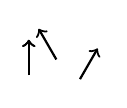
\begin{tikzpicture}
    \setfiguresize{-2.6}{-2.6}{+2.6}{+2.6}
    \begin{scope}[rotate=90]
        \drawevenhexgrid{-2}{-2}{5}{5}
        \drawdashedcounter{-2.00}{+0.00}{0}
        \drawdashedcounter{-1.00}{+0.00}{0}
        \drawaircraftcounter[90]{+0.00}{+0.00}{0}{F-4}{}{}
        \drawaircraftcounter[90]{+1.00}{-0.50}{30}{F-4}{}{}
        \drawdashedcounter{+2.00}{+0.00}{30}
        \begin{scope}[shift={(+0.20,+0.30)},thick,->]
            \miniathex{-2.00}{+0.00}{\draw (0:0.0) -- (0:0.45);}
            \miniathex{-1.00}{+0.00}{\draw (0:0.0) -- (0:0.45);}
        \end{scope}
        \begin{scope}[shift={(+0.40,-0.05)},thick,->]
            \miniathex{1.00}{-0.50}{\draw (30:0.0) -- (30:0.45);}
        \end{scope}
        \begin{scope}[shift={((0.15,-0.35))},thick,->]
            \miniathex{+0.00}{+0.00}{\draw [thick,->] (330:0.0) -- (330:0.45);}
        \end{scope}
        %\begin{scope}[shift={(0.0,+0.5)},anchor=east]
        %    \miniathex{-2.00}{+0.00}{\draw node {\minitable{r}{preparatory\\ HFP}};}
        %    \miniathex{-1.00}{+0.00}{\draw node {\minitable{r}{preparatory\\ HFP}};}
        %    \miniathex{+0.00}{+0.00}{\draw node {\minitable{r}{start\\ position}};}
        %    \miniathex{+1.00}{-0.50}{\draw node {\minitable{r}{roll\\ execution}};}
        %    \miniathex{+2.00}{+0.00}{\draw node {\minitable{r}{next\\ HFP}};}
        %\end{scope}
    \end{scope}
\end{tikzpicture}
\end{fitheight}
\hfil
\begin{fitheight}{5.2\standardhexwidth}
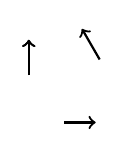
\begin{tikzpicture}
    \setfiguresize{-2.6}{-2.6}{+2.6}{+2.6}
    \begin{scope}[rotate=90]
        \drawoddhexgrid{-2}{-1.5}{5}{5}
        \drawdashedcounter{-2.00}{+0.00}{0}
        \drawdashedcounter{-1.00}{+0.00}{0}
        \drawaircraftcounter[90]{+0.00}{+0.00}{0}{F-4}{}{}
        \drawaircraftcounter[90]{+0.00}{-0.50}{30}{F-4}{}{}
        \drawdashedcounter{+1.00}{+0.00}{30}
        \begin{scope}[shift={(+0.20,+0.30)},thick,->]
            \miniathex{-2.00}{+0.00}{\draw (0:0.0) -- (0:0.45);}
            \miniathex{-1.00}{+0.00}{\draw (0:0.0) -- (0:0.45);}
        \end{scope}
        \begin{scope}[shift={(-0.40,-0.05)},thick,->]
            \miniathex{+0.00}{+0.00}{\draw (270:0.1) -- (270:0.5);}
        \end{scope}
        \begin{scope}[shift={(0.40,-0.60)},thick,->]
            \miniathex{+0.00}{+0.00}{\draw (30:0.0) -- (30:0.45);}
        \end{scope}
        \end{scope}
\end{tikzpicture}
\end{fitheight}


\figurecaption{figure:lag-roll-maneuvers}{Lag rolls to the right,each preceded by two preparatory HFPs and followed by another HFP. The execution of the roll is indicated by the counter images with solid borders. The number of preparatory FPs required depends on the aircraft speed and other factors.}

\end{twocolumnfigure}

}


}

\changedin{1C}{1C-figures}{
    \begin{FIGURE}
    \caption{Displacement Roll Maneuver}
    \medskip
    \includegraphics[width=0.8\linewidth]{figures/aids-displacement-roll.pdf}
    \end{FIGURE}
}{
    \begin{figure}[p]
\centering
\x{
\begin{tikzfigure}{1.0\linewidth}
\scriptsize

    \drawhexgrid[1]{11}{4.5}

    \begin{athex}{2.00}{0.00}
        \drawdashedcounter  {+0.00}{+1.00}{90}
        \drawaircraftcounter{+0.00}{+2.00}{90}{F-4}{}
        \drawaircraftcounter{+1.00}{+2.50}{90}{F-4}{}
        \drawdashedcounter  {+1.00}{+3.50}{90}
        \begin{scope}[shift={(135:0.3)},thick,->]
            \miniathex{0.00}{1.00}{\draw (90:0.1) -- (90:0.5);}
            \miniathex{1.00}{2.50}{\draw (90:0.1) -- (90:0.5);}
        \end{scope}
        \miniathex{+0.00}{+2.00}{\draw [thick,->] (30:0.35) -- (30:0.65);}
    \end{athex}

    \begin{athex}{3.50}{0.25}
        \drawdashedcounter{+0.50}{+0.75}{60}
        \drawaircraftcounter{+1.00}{+1.50}{60}{F-4}{}
        \drawaircraftcounter{+2.00}{+2.00}{60}{F-4}{}
        \drawdashedcounter{+2.50}{+2.75}{60}
        \begin{scope}[shift={(105:0.3)},thick,->]
            \miniathex{+0.50}{+0.75}{\draw (60:0.05) -- (60:0.4);}
            \miniathex{+2.00}{+2.00}{\draw (60:0.05) -- (60:0.4);}
        \end{scope}
        \miniathex{+1.00}{+1.50}{\draw [thick,->] (30:0.35) -- (30:0.65);}
    \end{athex}
    
    \begin{athex}{6.00}{0.00}
        \drawdashedcounter  {+0.50}{+0.75}{60}
        \drawaircraftcounter{+1.00}{+1.50}{60}{F-4}{}
        \drawaircraftcounter{+2.00}{+2.00}{60}{F-4}{}
        \drawdashedcounter  {+2.50}{+2.75}{60}
        \begin{scope}[shift={(105:0.3)},thick,->]
            \miniathex{+0.50}{+0.75}{\draw (60:0.05) -- (60:0.4);}
            \miniathex{+2.00}{+2.00}{\draw (60:0.05) -- (60:0.4);}
        \end{scope}
        \miniathex{+1.00}{+1.50}{\draw [thick,->] (30:0.35) -- (30:0.65);}
        \begin{scope}[shift={(315:0.5)},anchor=west]
            \miniathex{+0.50}{+0.75}{\draw node {start position};}
            \miniathex{+1.00}{+1.50}{\draw node {preparatory HFP};}
            \miniathex{+2.00}{+2.00}{\draw node {roll execution};}
            \miniathex{+2.50}{+2.75}{\draw node {next HFP};}
        \end{scope}
    \end{athex}

\end{tikzfigure}
\caption{Displacement Roll Maneuvers}
}{
\begin{tikzfigure}{1.0\linewidth}
\scriptsize

    \drawhexgrid[1]{11}{5.5}

    \begin{athex}{2.00}{1.00}
        \drawdashedcounter  {+0.00}{+0.00}{90}
        \drawdashedcounter  {+0.00}{+1.00}{90}
        \drawaircraftcounter{+0.00}{+2.00}{90}{F-4}{}
        \drawaircraftcounter{+1.00}{+2.50}{90}{F-4}{}
        \drawdashedcounter  {+1.00}{+3.50}{90}
        \begin{scope}[shift={(135:0.3)},thick,->]
            \miniathex{0.00}{0.00}{\draw (90:0.1) -- (90:0.5);}
            \miniathex{0.00}{1.00}{\draw (90:0.1) -- (90:0.5);}
            \miniathex{1.00}{2.50}{\draw (90:0.1) -- (90:0.5);}
        \end{scope}
        \miniathex{+0.00}{+2.00}{\draw [thick,->] (30:0.35) -- (30:0.65);}
    \end{athex}

    \begin{athex}{3.50}{1.25}
        \drawdashedcounter{+0.00}{+0.00}{60}
        \drawdashedcounter{+0.50}{+0.75}{60}
        \drawaircraftcounter{+1.00}{+1.50}{60}{F-4}{}
        \drawaircraftcounter{+2.00}{+2.00}{60}{F-4}{}
        \drawdashedcounter{+2.50}{+2.75}{60}
        \begin{scope}[shift={(105:0.3)},thick,->]
            \miniathex{+0.00}{+0.00}{\draw (60:0.05) -- (60:0.4);}
            \miniathex{+0.50}{+0.75}{\draw (60:0.05) -- (60:0.4);}
            \miniathex{+2.00}{+2.00}{\draw (60:0.05) -- (60:0.4);}
        \end{scope}
        \miniathex{+1.00}{+1.50}{\draw [thick,->] (30:0.35) -- (30:0.65);}
    \end{athex}
    
    \begin{athex}{6.00}{1.00}
        \drawdashedcounter  {+0.00}{+0.00}{60}
        \drawdashedcounter  {+0.50}{+0.75}{60}
        \drawaircraftcounter{+1.00}{+1.50}{60}{F-4}{}
        \drawaircraftcounter{+2.00}{+2.00}{60}{F-4}{}
        \drawdashedcounter  {+2.50}{+2.75}{60}
        \begin{scope}[shift={(105:0.3)},thick,->]
            \miniathex{+0.00}{+0.00}{\draw (60:0.05) -- (60:0.4);}
            \miniathex{+0.50}{+0.75}{\draw (60:0.05) -- (60:0.4);}
            \miniathex{+2.00}{+2.00}{\draw (60:0.05) -- (60:0.4);}
        \end{scope}
        \miniathex{+1.00}{+1.50}{\draw [thick,->] (30:0.35) -- (30:0.65);}
        \begin{scope}[shift={(315:0.5)},anchor=west]
            \miniathex{+0.00}{+0.00}{\draw node {start position};}
            \miniathex{+0.50}{+0.75}{\draw node {preparatory HFP};}
            \miniathex{+1.00}{+1.50}{\draw node {preparatory HFP};}
            \miniathex{+2.00}{+2.00}{\draw node {roll execution};}
            \miniathex{+2.50}{+2.75}{\draw node {next HFP};}
        \end{scope}
    \end{athex}
    
\end{tikzfigure}
\caption{Displacement rolls to the right, each with two preparatory HFPs. The number of preparatory HFPs required depends on the aircraft speed and other factors.}
}
\label{figure:displacement-roll-maneuvers}
\end{figure}

}

\changedin{1C}{1C-figures}{
    \begin{FIGURE}
    \caption{Barrel Roll Maneuver}
    \medskip
    \includegraphics[width=0.6\linewidth]{figures/aids-barrel-roll.pdf}
    \end{FIGURE}
}{
    \begin{onecolumnfigure}[tbp]
\CX{
\begin{fitwidth}{7.333\standardhexwidth}
\begin{tikzpicture}

\scriptsize

    \drawhexgrid{0}{0}{6}{5}

    \begin{athex}{0.00}{0.00}
        \drawdashedcounter  {+0.50}{+0.75}{60}
        \drawaircraftcounter{+1.00}{+1.50}{60}{F-4}{}{}
        \drawaircraftcounter{+2.00}{+2.00}{90}{F-4}{}{}
        \begin{scope}[shift={(105:0.3)},thick,->]
            \miniathex{+0.50}{+0.75}{\draw (60:0.05) -- (60:0.4);}
        \end{scope}
        \miniathex{+1.00}{+1.50}{\draw [thick,->] (30:0.35) -- (30:0.65);}
        \begin{scope}[shift={(315:0.5)},anchor=west]
            \miniathex{+0.50}{+0.75}{\draw node {start position};}
            \miniathex{+1.00}{+1.50}{\draw node {preparatory HFP};}
            \miniathex{+2.00}{+2.00}{\draw node {first roll execution};}
            \miniathex{+2.00}{+3.00}{\draw node {preparatory HFP};}
            \miniathex{+3.00}{+3.50}{\draw node {second roll execution};}
            \miniathex{+3.00}{+4.25}{\draw node {preparatory HFP};}
            \miniathex{+3.00}{+5.00}{\draw node {third roll execution};}
        \end{scope}
        \begin{scope}[shift={(345:0.5)},anchor=west]
        \end{scope}
    \end{athex}

    \begin{athex}{2.00}{1.00}
        \drawaircraftcounter{+0.00}{+2.00}{90}{F-4}{}{}
        \drawaircraftcounter{+1.00}{+2.50}{120}{F-4}{}{}
        \begin{scope}[shift={(135:0.3)},thick,->]
            \miniathex{0.00}{1.00}{\draw (90:0.1) -- (90:0.5);}
        \end{scope}
        \begin{scope}[shift={(30:0.2)}]
            \miniathex{+0.00}{+2.00}{\draw [thick,->] (0:0.25) -- (0:0.65);}
        \end{scope}
    \end{athex}

    \begin{athex}{3.50}{2.75}
        \drawaircraftcounter{-1.00}{+1.50}{120}{F-4}{}{}
        \drawaircraftcounter{-0.50}{+1.75}{150}{F-4}{}{}
        \begin{scope}[shift={(165:0.3)},thick,->]
            \miniathex{-0.50}{+0.75}{\draw (120:0.05) -- (120:0.4);}
        \end{scope}
        \begin{scope}[shift={(315:0.4)},thick,->]
            \miniathex{-1.00}{+1.50}{\draw (30:0.1) -- (30:0.5);}
        \end{scope}
    \end{athex}
    
\end{tikzpicture}
\end{fitwidth}

\figurecaption{figure:barrel-roll-maneuvers}{Barrel Roll Maneuvers.}

}{
\begin{fitheight}{9.2\standardhexwidth}
\begin{tikzpicture}
\scriptsize

    \setfiguresize{-2.6}{-4.6}{+6.1}{+4.6}
    \drawevenhexgrid{-2}{-4}{9}{9}

    \begin{athex}{-1.00}{-3.50}
        \drawdashedcounter  {+0.00}{+0.00}{60}
        \drawdashedcounter  {+0.50}{+0.75}{60}
        \drawaircraftcounter{+1.00}{+1.50}{60}{F-4}{}{}
        \drawaircraftcounter{+2.00}{+2.00}{90}{F-4}{}{}
        \begin{scope}[shift={(105:0.3)},thick,->]
            \miniathex{+0.50}{+0.75}{\draw (60:0.05) -- (60:0.4);}
        \end{scope}
        \begin{scope}[shift={(135:0.3)},thick,->]
            \miniathex{+2.00}{+2.00}{\draw (90:0.1) -- (90:0.5);}
        \end{scope}
        \miniathex{+1.00}{+1.50}{\draw [thick,->] (30:0.35) -- (30:0.65);}
        \begin{scope}[shift={(315:0.5)},anchor=west]
            \miniathex{+0.00}{+0.00}{\draw node {start position};}
            \miniathex{+0.50}{+0.75}{\draw node {preparatory HFP};}
            \miniathex{+1.00}{+1.50}{\draw node {preparatory HFP};}
            \miniathex{+2.00}{+2.00}{\draw node {first roll execution};}
            \miniathex{+2.00}{+3.00}{\draw node {preparatory HFP};}
            \miniathex{+2.00}{+4.00}{\draw node {preparatory HFP};}
            \miniathex{+3.00}{+4.50}{\draw node {second roll execution};}
        \end{scope}
        \begin{scope}[shift={(345:0.5)},anchor=west]
            \miniathex{+2.50}{+5.25}{\draw node {preparatory HFP};}
            \miniathex{+2.00}{+6.00}{\draw node {preparatory HFP};}
            \miniathex{+2.00}{+7.00}{\draw node {third roll execution};}
        \end{scope}
    \end{athex}
    
    \begin{athex}{1.00}{-1.50}
        \drawdashedcounter  {+0.00}{+1.00}{90}
        \drawaircraftcounter{+0.00}{+2.00}{90}{F-4}{}{}
        \drawaircraftcounter{+1.00}{+2.50}{120}{F-4}{}{}
        \begin{scope}[shift={(135:0.3)},thick,->]
            \miniathex{0.00}{1.00}{\draw (90:0.1) -- (90:0.5);}
        \end{scope}
        \begin{scope}[shift={(165:0.3)},thick,->]
            \miniathex{1.00}{2.50}{\draw (120:0.05) -- (120:0.4);}
        \end{scope}
        \begin{scope}[shift={(30:0.2)}]
            \miniathex{+0.00}{+2.00}{\draw [thick,->] (0:0.25) -- (0:0.65);}
        \end{scope}
    \end{athex}

    \begin{athex}{2.00}{1.00}
        \drawdashedcounter  {-0.50}{+0.75}{120}
        \drawaircraftcounter{-1.00}{+1.50}{120}{F-4}{}{}
        \drawaircraftcounter{-1.00}{+2.50}{120}{F-4}{}{}
        \begin{scope}[shift={(165:0.3)},thick,->]
            \miniathex{-0.50}{+0.75}{\draw (120:0.05) -- (120:0.4);}
        \end{scope}
        \begin{scope}[shift={(45:0.3)},thick,->]
            \miniathex{-1.00}{+1.50}{\draw (90:0.1) -- (90:0.5);}
        \end{scope}
    \end{athex}

\end{tikzpicture}
\end{fitheight}

\figurecaption{figure:barrel-roll-maneuvers}{A barrel roll executed as a sequence of two lag rolls to the right followed by one displacement roll to the right, each with two preparatory HFPs. Any combination of lag rolls and displacement rolls may make up a barrel roll, but all must be in the same direction. The number of preparatory FPs required before each roll depends on the aircraft speed and other factors.}
}

\end{onecolumnfigure}

}

\addedin{2A}{2A-missile-attacks}{
    \begin{FIGURE}[tb]

\begin{tikzfigure}{9.333\standardhexwidth}

    \drawhexgrid{0}{0}{8}{2}  

    \begin{athex}{7.00}{0.50}
        \drawdotathex{+0.00}{0.50}
        \drawdotathex{-0.50}{0.75}
        \drawdotathex{+0.50}{0.75}
        \drawdotathex{+0.00}{1.00}
        \drawdotathex{-0.50}{1.25}
        \drawdotathex{+0.50}{1.25}
        \drawdotathex{+0.00}{1.50}
        \drawarrowcounter{0.00}{0.00}{90}
    \end{athex}

    \begin{athex}{1.00}{0.50}
        \drawdotathex{+0.00}{0.50}
        \drawdotathex{+0.00}{1.00}
        \drawdotathex{+0.50}{0.25}
        \drawdotathex{+0.50}{0.75}
        \drawdotathex{+0.50}{1.25}
        \drawdotathex{+1.00}{0.50}
        \drawdotathex{+1.00}{1.00}
        \drawarrowcounter{0.00}{0.00}{60}
    \end{athex}

    \begin{athex}{3.50}{0.25}
        \drawdotathex{+0.00}{0.50}
        \drawdotathex{+0.00}{1.00}
        \drawdotathex{+0.50}{0.25}
        \drawdotathex{+0.50}{0.75}
        \drawdotathex{+0.50}{1.25}
        \drawdotathex{+1.00}{0.50}
        \drawdotathex{+1.00}{1.00}
        \drawarrowcounter{0.00}{0.00}{60}
    \end{athex}
    
\end{tikzfigure}

\CAPTION{figure:missile-attacks}{\protect\x{Air-to-Air Missile Attacks}{A missile attacks when it passes through the target hex at its altitude or when is co-altitude with the target, has at least one FP remaining in the proportional move, and the target occupies one of the positions show above.}}

\end{FIGURE}

}

\changedin{1C}{1C-figures}{
    \begin{FIGURE*}
    \caption{Jamming Cell Formations}
    \medskip
    \includegraphics[width=0.6\linewidth]{figures/aids-jamming-cells.pdf}
    \medskip
    \begin{minipage}{0.6\linewidth}
    \addedin{1B}{1B-apj-23-errata}{
    \begin{enumerate}
        \item To be in a valid Jamming Cell formation, aircraft must be in adjacent hexes (as depicted), with no more than 30 degrees difference in facing and within 1 altitude level of an adjacent aircraft.
        \item The maximum size of a jamming cell is 4 aircraft. Each aircraft within those parameters has its ECM jammer rating increased by 1.
    \end{enumerate}}
    \end{minipage}
    \end{FIGURE*}
}{
    \newcommand{\drawjammingcellhex}[2]{
    \drawhex[black!10]{#1}{#2}
}

\newcommand{\drawjammingcellaircraft}[3]{
    \drawaircraftcounter{#1}{#2}{#3}{F-105}{}
}

\newcommand{\drawjammingcellhexandaircraft}[3]{
    \drawjammingcellhex{#1}{#2}
    \drawjammingcellaircraft{#1}{#2}{#3}
}

\begin{tikzfigure}{\linewidth}
    \drawhexgrid{12}{10}

    \drawjammingcellhexandaircraft{1.0}{1.5}{90}
    \drawjammingcellhexandaircraft{2.0}{1.0}{90}
    \drawjammingcellhexandaircraft{2.0}{2.0}{90}
    \drawjammingcellhexandaircraft{3.0}{1.5}{90}

    \drawjammingcellhexandaircraft{5.0}{1.5}{120}
    \drawjammingcellhexandaircraft{6.0}{2.0}{120}
    \drawjammingcellhexandaircraft{7.0}{2.5}{120}
    \drawjammingcellhexandaircraft{8.0}{3.0}{120}
    
    \drawjammingcellhexandaircraft{8.0}{1.0}{90}
    \drawjammingcellhexandaircraft{9.0}{1.5}{90}
    \drawjammingcellhexandaircraft{10.0}{1.0}{90}
    \drawjammingcellhexandaircraft{11.0}{1.5}{90}
    
    \drawjammingcellhexandaircraft{1.0}{4.5}{120}
    \drawjammingcellhexandaircraft{1.0}{5.5}{120}
    \drawjammingcellhexandaircraft{2.0}{5.0}{120}
    
    \drawjammingcellhexandaircraft{4.0}{5.0}{90}
    \drawjammingcellhexandaircraft{5.0}{5.5}{90}
    \drawjammingcellhexandaircraft{6.0}{5.0}{90}
    
    \drawjammingcellhexandaircraft{8.0}{5.0}{90}
    \drawjammingcellhexandaircraft{9.0}{5.5}{90}
    \drawjammingcellhexandaircraft{10.0}{6.0}{90}
    
    \drawjammingcellhexandaircraft{1.0}{7.5}{120}
    \drawjammingcellhexandaircraft{2.0}{8.0}{120}
    
    \drawjammingcellhexandaircraft{4.0}{8.0}{90}
    \drawjammingcellhexandaircraft{5.0}{8.5}{90}
    
    \drawjammingcellhex{7.0}{8.5}
    \drawjammingcellhex{8.0}{9.0}
    \drawjammingcellaircraft{6.5}{8.25}{120}
    \drawjammingcellaircraft{8.5}{9.25}{120}
    
    \drawjammingcellhexandaircraft{10.0}{8.0}{120}
    \drawjammingcellhexandaircraft{11.0}{7.5}{120}

    \draw (0.75,3.00) node [anchor=west, fill=white, draw=black] {Four-Aircraft Cells};
    \draw (0.75,6.50) node [anchor=west, fill=white, draw=black] {Three-Aircraft Cells};
    \draw (0.75,9.00) node [anchor=west, fill=white, draw=black] {Two-Aircraft Cells};

\end{tikzfigure}

}

\changedin{1C}{1C-figures}{
    \begin{FIGURE}
    \caption{Crash Site Determination}
    \medskip
    \includegraphics[width=1.0\linewidth]{figures/aids-crash-site.pdf}
    \end{FIGURE}
}{
    \begin{figure}[tbp]
\centering
\begin{tikzfigure}{1.0\linewidth}

    \drawhexgrid{13}{6}

    \newcommand{\drawcrashhex}[3]{
        \miniathex{#1}{#2}{
            \drawhex[black!10]{0}{0}
            \draw node {#3};
        }
    }

    \begin{athex}{2.00}{1.00}
        \drawcrashhex{+0}{+1.0}{1}
        \drawcrashhex{-1}{+1.5}{2}
        \drawcrashhex{+0}{+2.0}{3}
        \drawcrashhex{+1}{+1.5}{4}
        \drawcrashhex{-1}{+2.5}{5}
        \drawcrashhex{+0}{+3.0}{6}
        \drawcrashhex{+1}{+2.5}{7}
        \drawcrashhex{-1}{+3.5}{8}
        \drawcrashhex{+0}{+4.0}{9}
        \drawcrashhex{+1}{+3.5}{10}
        \drawaircraftcounter{0.00}{0.00}{90}{F-4}{}
    \end{athex}

    \begin{athex}{5.00}{1.50}
        \drawcrashhex{+0}{+1.0}{1}
        \drawcrashhex{+1}{+0.5}{2}
        \drawcrashhex{+0}{+2.0}{3}
        \drawcrashhex{+1}{+1.5}{4}
        \drawcrashhex{+2}{+1.0}{5}
        \drawcrashhex{+1}{+2.5}{6}
        \drawcrashhex{+2}{+2.0}{7}
        \drawcrashhex{+1}{+3.5}{8}
        \drawcrashhex{+2}{+3.0}{9}
        \drawcrashhex{+3}{+2.5}{10}
        \drawaircraftcounter{0.00}{0.00}{60}{F-4}{}
    \end{athex}

    \begin{athex}{9.50}{1.25}
        \drawcrashhex{-0.5}{+1.25}{1}
        \drawcrashhex{+0.5}{+0.75}{2}
        \drawcrashhex{+1.5}{+0.25}{3}
        \drawcrashhex{+0.5}{+1.75}{4}
        \drawcrashhex{+1.5}{+1.25}{5}
        \drawcrashhex{+0.5}{+2.75}{6}
        \drawcrashhex{+1.5}{+2.25}{7}
        \drawcrashhex{+2.5}{+1.75}{8}
        \drawcrashhex{+1.5}{+3.25}{9}
        \drawcrashhex{+2.5}{+2.75}{10}
        \drawaircraftcounter{0.00}{0.00}{60}{F-4}{}
    \end{athex}    
    
\end{tikzfigure}
\caption{Crash Sites}
\label{figure:crash-sites}
\end{figure}

}

\begin{table}
\centering
\caption{Air to Air Gun and Rocket Attack Modifiers}
\medskip
\begin{tabular}{ll}
\hline
\multicolumn{2}{c}{Aircraft}\\
\hline
Firer Snap Shooting&$+1$\\
Firer L or 2L damaged&$+1$\\
Firer H damaged&$+2$\\
Firer C damaged&$+3$\\
RE Radar Ranging&$-1$\\
CA Radar Ranging&$-2$\\
IG Radar Ranging&$-3$\\
Each 1/3d FPs on SSGT&$-1$\\
Target Aircraft Size&Var. $+,-$\\
Gunsight Turn Rate&Var. $+,-$\\
\hline
\multicolumn{2}{c}{Angle-Off}\\
\hline
0 line&$-2$\\
30 Arc&$+0$\\
60 Arc&$+2$\\
90 Arc&$+4$\\
120 Arc&$+4$\\
150 Arc&$+4$\\
180 Arc&$+3$\\
180 line&$+2$\\
Vertical Attack&$+2$\\
\hline
Pilot\\
\hline
Veteran&$-1$\\
Combat Hero&$-1$\\
Novice&$+1$\\
Green&$+2$\\
\hline
\end{tabular}
\end{table}
\begin{onecolumntable}

\tablecaption{table:cummulative-damage}{Cumulative Hits Effects}

\begin{tabular}{l@{ }c@{ }l}
\hline
Three L&=&H Damage\\
Two H&=&C Damage\\
Two C&=&K Aircraft Killed\\
C + H&=&K Aircraft Killed\\
\hline
\end{tabular}

\end{onecolumntable}
\begin{TABLE}

\TABLECAPTION{table:progressive-damage}{Progressive Damage}
\medskip
\begin{tabular}{ccc}
\hline
\minitable{c}{Current\\Damage}&
\minitable{c}{Die Roll\\or less}&
\minitable{c}{Increased\\Damage}\\
\hline
L or 2L&2&H\\
H&3&C\\
C&4&K\\
\hline
\end{tabular}

\end{TABLE}
\begin{TABLE}

\TABLECAPTION{table:aircraft-damage}{Aircraft Damage}

\begin{tabularx}{0.8\linewidth}{X*{10}{@{ }c@{ }}}
\hline
\multirow{2}{*}{\minitable{c}{Die\\Roll}}&
\multicolumn{10}{c}{Weapon Attack Rating}\\
&1&2&3&4&5&6&7&8&9&10\\
\hline
$0-$&K&K&K&K&K&K&K&K&K&K\\
1&C&C&K&K&K&K&K&K&K&K\\
2&H&H&C&K&K&K&K&K&K&K\\
3&L&H&H&C&K&K&K&K&K&K\\
4&L&L&H&H&C&C&K&K&K&K\\
5&L&L&2L&H&C&C&C&K&K&K\\
6&L&L&L&H&H&C&C&C&K&K\\
7&---&L&L&L&H&H&C&C&C&K\\
8&---&---&L&L&2L&H&H&H&C&C\\
9&---&---&---&L&L&2L&H&H&H&C\\
$10+$&---&---&---&---&L&L&2L&H&H&H\\
\hline
&\phantom{2L}&\phantom{2L}&\phantom{2L}&\phantom{2L}&\phantom{2L}&\phantom{2L}&\phantom{2L}&\phantom{2L}&\phantom{2L}&\phantom{2L}\\[-3ex]
\end{tabularx}

\medskip

\begin{tablenote}{0.8\linewidth}
Damage Modifiers
\medskip

\begin{itemize}
    \item Shift one column right if aircraft already L or more damaged.
    \item Shift one column left if hit was from gun snap shot.
    \item $-2$ to die roll if air to air rocket hit or direct hit from missile.
    \item Plus or Minus Aircraft Vulnerability as listed on target ADC.
\end{itemize}

\end{tablenote}

\end{TABLE}
\begin{table}
\centering
\caption{Air to Air Rocketry}
\medskip
\begin{tabular}{lcccccccccc}
\hline
\multirow{2}{*}{\minitable{c}{Range\\to TGT}}&
\multicolumn{10}{c}{Total Rocket Factors Fired}\\
&1&2&3&4&5&6&7&8&9&10\\
\hline
1&1&2&2&3&3&4&4&5&6&6\\
2&1&2&2&2&2&3&3&4&4&5\\
3&0&1&1&1&2&2&2&2&3&3\\
4&0&0&1&1&1&1&2&2&2&2\\
\hline
\tablemedskip
\tablenotes{11}{0.75\linewidth}{
(above = die roll to hit numbers)

\medskip
Rocketry modifiers
\medskip

\begin{enumerate}[nosep]
    \item If C.C. Rocket Attack Technology in effect, apply a $-2$ modifier to the hit roll.
    \item All other gun and rocket attack modifiers apply as well.
\end{enumerate}

\medskip
C.C. Rocket Attack Procedure:
\medskip

Target must be locked-on by radar, and firer may only use TT or less turns, altitude changes of no more than 1 level and no maneuvers except slides up to the point of firing.
}
\end{tabular}
\end{table}
\begin{onecolumntablefloat}[t!]
\begin{onecolumntable}
\tablecaption{table:aircraft-damage-effects}{Aircraft Damage Effects}
\x{
\begin{tabularx}{\linewidth}{cX}
\toprule
\minitable{c}{Damage}&
Effect\\
\midrule
---&Superficial Damage; no adverse effects.\\
L&Light Damage; no ET turns allowed; lose High Pitch Rate; aircraft becomes Low Roll Rate\\
2L&Light Damage; as L plus no BT turns allowed, $+1$ to all preparatory move requirements.\\
H&Heavy Damage; as 2L plus Mil and A/B power halved, CCC halved, no roll maneuvers allowed, no supersonic flight allowed. Roll once for Systems loss.\\
C&Crippled; as H plus lose A/B power, no HT turns, aircraft smokes, lose all technology. Roll again for Systems loss.\\
K&Aircraft Killed (shot down), remove from play.\\
\bottomrule
\end{tabularx}
\begin{tablenote}{\linewidth}
Note: if end speed > High Transonic when “H” or “C” damaged, roll twice for prog.\ damage even if Damage Control done.
\end{tablenote}
}{
\begin{tabularx}{\linewidth}{cX}
\toprule
Damage&
\multicolumn{1}{c}{Effects}\\
\midrule
\addlinespace
L&The aircraft can no longer turn at the ET rate, loses HPR, and becomes LRR.\\
\addlinespace
&The aircraft suffers a $+1$ modifier to air-to-air gun and rocket attacks and to weapon launches.\\
\addlinespace
2L&As L, and additionally the aircraft can no longer turn at the BT rate and requires an additional preparatory FP before all maneuvers.\\
\addlinespace
&The aircraft suffers a $+1$ modifier to air-to-air gun and rocket attacks and to weapon launches.\\
\addlinespace
H&As 2L, and additionally the aircraft receives only half of the normal APs from military and afterburner, has its CC halved, and will potentially suffer damage if it uses supersonic speeds.\\
\addlinespace
&The aircraft must check for a system loss.\\
\addlinespace
&The aircraft suffers a $+2$ modifier to air-to-air gun and rocket attacks and to weapon launches.\\
\addlinespace
C&As H, and additionally the aircraft loses afterburner power, can no longer turn at the HT rate, smokes, and loses all technology.\\
\addlinespace
&The aircraft must check for a system loss.\\
\addlinespace
&The aircraft suffers a $+3$ modifier to air-to-air gun and rocket attacks and to weapon launches.\\
\addlinespace
K&The aircraft is destroyed and removed from play.\\
\addlinespace
&The crew may attempt emergency egress (rule~\ref{rule:emergency-egress}).\\
\addlinespace
\bottomrule
\end{tabularx}

}
\end{onecolumntable}
\end{onecolumntablefloat}
\input{tables/table-systems-loss}
\addedin{1B}{1B-apj-22-damage-tables}{

\begin{twocolumntable}
\x{

\tablecaption{table:optional-damage}{Optional Advanced Aircraft Damage}
\small
\begin{tabularx}{\linewidth}{lcX}
\toprule
\multirow{2}{*}{\minitable{c}{Die\\Roll}}&
\multirow{2}{*}{\minitable{c}{Hit\\Location}}&
Damage Effects to Aircraft and Notes\\
\\
\midrule
\multicolumn{3}{c}{Light Damage}\\
\midrule
&&$+1$ to all attacks, $+1$ to weapons launches.\\
1&Airframe&No supersonic speeds allowed.$^*$\\
2&Airframe&No BT or ET turn rate allowed.\\
3&Controls&Aircraft becomes Low roll rate and loses any high pitch rate capability.\\
4&Controls&Add one to prep-move requirements for all maneuvers.\\
5&Fuel&Lose 1 point of fuel per game turn, double bingo fuel amount. White Vapor emitted.\\
6&Avionics&Radar knocked out and lose all technology.\\
7&Avionics&Bombsight degraded to manual, gunsight = TT+1, HT+2, BT+3.\\
8&Weapons&Internal guns/gun pods disabled.\\
9&Engines&Afterburner disabled. No A/B power available.\\
10&Engines&Thrust loss; reduce Mil and A/B power numbers by 0.5. White Vapor emitted.\\
\midrule
\multicolumn{3}{c}{Heavy Damage}\\
\midrule
&&+2 to all attacks, +2 to weapon launches.\\
1,2&Airframe&No supersonic flight.$^*$ No BT or ET turns. Low roll rate. No high pitch rate. Add two to prep-move requirements for all maneuvers.\\
3&Controls&No rolling maneuvers allowed. Low roll rate. No high pitch rate. No ET turn rate.\\
4&Controls&Throttle jammed, no power changes. No HT, BT, or ET turn rate. No high pitch rate.\\
5&Fuel&Lose 2 points of fuel per turn. Bingo fuel tripled. Roll one die each turn after flight. On 1, a FUEL FIRE occurs (see description below). Aircraft becomes Smoker.\\
6,7&Avionics&Radar knocked out, all ECM knocked out, and lose all technology\\
8&Weapons&Guns disabled, no RHM/AHM/ARM/ASM missile or BS/RS weapon launches allowed.\\
9,10&Engines&Mil and A/B power halved. Roll for flame out whenever power setting changed. On 1, a Flame-Out occurs in one good engine. Aircraft becomes a smoker.\\
\midrule
\multicolumn{3}{c}{Critical Damage}\\
\midrule
&&$+3$ to all attacks, $+3$ to weapon launches. Roll once on the H table and once below.\\
1&Cockpit&Roll die again: 1, 2 = pilot killed (aircraft lost). 3, 4 = Crewman Killed (lose multi-crew functions). +5 = crew okay. Regardless, treat aircraft as having both an Airframe and Avionics hit as described immediately below.\\
2,3&Airframe&
No supersonic flight.$^*$ Low roll rate. No high pitch. No rolling maneuvers. EZ turns only. Aircraft must jettison external stores.\\
4,5,6&Avionics&Lose radar, all ECM, and all technology. No external pods work. Bombsight degrades to manual and gunsight = TT+1, HT+2, BT+3.\\
7&Fuel Fire**&Aircraft becomes Smoker. Lose 3 die rolls of fuel/turn. Jettison external stores. Roll die after each turn after flight. On 1 or 2 aircraft explodes, crew killed. On 9 or 10, fire goes out permanently but fuel leak still there.\\
8,9,10&Engines&A/B power lost. Mil power halved. Aircraft becomes Smoker. Roll for flame-outs twice per engine (1 or 2 = F.O. in this case). On subsequent turns, roll for flame-out whenever power seting is changed (1 = F.O.).\\
\bottomrule
\end{tabularx}
\begin{tablenote}{\linewidth}
\begin{itemize}
    \item The specifics of the damage rolled are not revealed to the enemy, but are recorded on paper. Visible signs of damage such as smoke or vapor, as indicated on the tables, must be told to the opponent.
    \item Jettison of Stores: Only the results calling for jettison of ordnance require an aircraft to do so. If this is the case, the aircraft must jettison enough stores to become CL configured. 
    \item If table indicates damage to a system or performance capability that the aircraft does not have, roll again. If the second roll also results in non-applicable damage, the hit is still recorded for the die roll penalties on combat and for possible progressive damage.
   \item[$^*$] If supersonic speeds exceeded in game turn, roll for progressive damage twice even if Damage Control was done.
   \item[$^{**}$] A Fuel Fire and risk of explosion can only be stopped by shutting down all engines. Declare this when doing damage control. Treat aircraft as flamed-out. When engines relit, A/B is disabled. Roll one die, on 1 to 4 fire resumes permanently; otherwise it stays out.
\end{itemize}
\end{tablenote}
\end{twocolumntable}

}{

\tablecaption{table:optional-damage}{Optional Aircraft Damage}
\small
\begin{tabularx}{\linewidth}{ccX}
\toprule
\multirow{2}{*}{\minitable{c}{Die\\Roll}}&
\multirow{2}{*}{\minitable{c}{Hit\\Location}}&
\multicolumn{1}{c}{\multirow{2}{*}{Effects}}
\\
\\
\midrule
\multicolumn{3}{c}{L or 2L Damage}\\
\midrule
&&$+1$ to all attacks and weapons launches.
\\
\cmidrule{3-3}
1&Airframe&
The aircraft must check twice for progressive damage at supersonic speeds.
\\
2&Airframe&
The aircraft may not use the BT or ET turn rates.
\\
3&Controls&
The aircraft becomes LRR and loses any HPR capability.
\\
4&Controls&
The aircraft requires one additional preparatory FP before all maneuvers.
\\
5&Fuel&
The aircraft loses 1 fuel point per game turn. 
Its bingo fuel level is doubled.
It emits a white vapor.
\\
6&Avionics&
The aircraft's radar and technology are disabled.
\\
7&Avionics&
The aircraft's bombsight is degraded to manual, and its gunsight to TT +1, HT +2, and BT +3.
\\
8&Weapons&
The aircraft can no longer use internal guns or gun pods.
\\
9&Engines&
The aircraft can no longer use afterburner power.
\\
10&Engines&
The aircraft's thrust at military and afterburner power is reduced by 0.5 AP.
It emits a white vapor.
\\
\midrule
\multicolumn{3}{c}{H Damage}\\
\midrule
&&+2 to all attacks and weapon launches.\\
\cmidrule{3-3}
1 or 2&Airframe&
The aircraft must check twice for progressive damage at supersonic speeds.
It may not use the BT or ET turn rates.
It becomes LRR and loses any HPR capability.
It requires two additional preparatory FP before all maneuvers.
\\
3&Controls&
The aircraft may not perform rolling maneuvers. 
It becomes LRR and loses any HPR capability.
It may not use the ET turn rate.
\\
4&Controls&
The aircraft's throttle jams. 
It may not change its power setting.
It may not use the HT, BT, or ET turn rates.
It loses any HPR capability.
\\
5&Fuel&
The aircraft loses 2 fuel points per game turn. 
Its bingo fuel level is tripled. 
It becomes a smoker.
The aircraft must check each game turn after flight for a fuel fire. On a die roll of $1-$, a fire starts.
\\
6 or 7&Avionics&
The aircraft's radar, ECM, and technology are disabled.
\\
8&Weapons&
The aircraft can no longer use internal guns or gun pods or launch RHM/AHM/ARM/ASM missiles or BS/RS weapons.
\\
9 or 10&Engines&
The aircraft's thrust at military and afterburner power is reduced to one-half the normal values.
It must check for a flame-out each time it changes its power setting. On a $1-$, one good engine flames out.
The aircraft becomes a smoker.
\\
\midrule
\multicolumn{3}{c}{C Damage}\\
\midrule
&&Roll once on the H table and once on the C table.\\
&&$+3$ to all attacks and weapon launches.\\
\cmidrule{3-3}
1&Cockpit&
Roll the die again: 1 or 2 = pilot killed (equivalent to K). 3 or 4 = crewmember killed (lose multi-crew functions). $5+$ = crew unhurt. 
Treat the aircraft as having both the airframe and avionics results described immediately below.
\\
2 or 3&Airframe&
The aircraft must check twice for progressive damage at supersonic speeds.
It may only use the EZ turn rate.
It becomes LRR and loses any HPR capability.
It may not perform rolling maneuvers. 
It must jettison stores.
\\
4 to 6&Avionics&
The aircraft's radar, ECM, technology, and all external pods are disabled.
Its bombsight is degraded to manual, and its gunsight to TT +1, HT +2, and BT +3.
\\
7&Fuel&
The aircraft suffers a fuel fire.
It loses 3 fuel points per game turn. 
%Its bingo fuel level is quadrupled. 
It becomes a smoker.
It must jettison stores.
%Roll die after each turn after flight. On 1 or 2 aircraft explodes, crew killed. On 9 or 10, the fire goes out permanently, but the fuel leak is still there.
\\
8 to 10&Engines&
The aircraft loses afterburner power, and its thrust at military power is reduced to one-half the normal value.
It becomes a smoker.
It immediately checks twice per engine for a flame-out on a $2-$. On subsequent turns, if it changes its power setting, each engine flames out on a $1-$.
\\
\bottomrule
\end{tabularx}

}

\end{twocolumntable}

}


\clearpage

\begin{table}
\centering
\caption{Air to Air Missile Launch Modifiers}
\medskip
\begin{tabular}{p{20em}l}
\hline
\multicolumn{2}{c}{IR Missiles}\\
\hline
Each Turn Rate over Launch Gee&$+2$\\
Fired from LO or ML alt.\ band at lower target&$+2$\\
Fired into sun clutter&$+3$\\
Fired out-of-enveloped&$+3$\\
Fired at lower target above highest cloud layer&$+3$\\
Lesser of Flare PPL or missile Flare Vulnerability number if DDS program is in effect.&$+$\\
\hline
\multicolumn{2}{c}{BR, RH, and AH Missiles}\\
\hline
Each Turn Rate over Launch Gee&$+2$\\
Snap Fired&$+3$\\
Fired out-of-enveloped&$+3$\\
\hline
\multicolumn{2}{c}{Crew}\\
\hline
Veteran&$-1$\\
Combat Hero, 
Tactics Master or both&$-1$\\
Green&$+1$\\
\hline
\multicolumn{2}{c}{Damage}\\
\hline
L or 2L&$+1$\\
H&$+2$\\
C&$+2$\\
\hline
\end{tabular}
\end{table}
\begin{table}
\centering
\caption{Air to Air Missile and SAM Attack Modifiers}
\medskip
\begin{tabular}{p{20em}l}
\hline
\multicolumn{2}{c}{IRMs and IR SAMs}\\
\hline
Target in Afterburner Power&$-3$\\
Target in Military Power&$-2$\\
Target in Idle Power&$+1$\\
Missile must lose 2 or more levels during proportional move of attack against tgt.\ in LO alt.\ band (ground clutter)&$+2$\\
Target in Terrain Following Flight&$+1$\\
Lesser of Flare PPL or missile Flare Vulnerability no.&$+$\\
\hline
\multicolumn{2}{c}{BRMs, RHMs, AHMs, \& BR, CG, CW and TVM SAMs}\\
\hline
DJM rating $-$ missile ECCM$+$\\
Lesser of Chaff PPL or missile Chaff Vulnerability&$+$\\
Lesser of Mini-jammer PPL or Chaff Vulnerability $+$ 1&$+$\\
Ground clutter (air to air missiles only) = $6 - \text{target Altitude above terrain} - \text{missile ECCM}$.&$+$\\
Listed “T” level modifier (SAMs only, if applicable)&$+$\\
\hline
\multicolumn{2}{c}{OG and LG SAMs}\\
\hline
\multicolumn{2}{l}{No modifiers other than angle-off and aircraft size apply.}\\
\hline
\multicolumn{2}{c}{ALL Missiles}\\
\hline
Target aircraft size modifier from ADC&$+/-$\\
Target did not engage the missile&$-1$\\
\hline
\tablemedskip
\tablenotes{2}{0.9\linewidth}{
Reminder: $\text{Max launch range for \changedin{1B}{1B-apj-23-errata and 1B-apj-24-play-aids}{RHM/AHM}{RHM}} = 3 \times \text{radar Track Str.\ \#}$.
}
\end{tabular}

\bigskip

\caption{Missile Angle-Off Modifiers to Attack}
\medskip
\begin{tabular}{lccccccc}
\hline
\multirow{2}{*}{\minitable{c}{Angle-Off\\Arc}}&\multicolumn{7}{c}{Missile Seeker Type}\\
&E&I&M&A&BR&RH&AH\\
\hline
0 line        &$-1$&$-1$&$-1$&$-2$&$+0$&$-1$&$-2$\\
30 arcs       &$+0$&$+0$&$+0$&$+0$&$+0$&$+0$&$+0$\\
60 arcs       &$+1$&$+0$&$+0$&$+0$&$+1$&$+0$&$+0$\\
90/120 arcs   &$+3$&$+2$&$+2$&$+2$&$+3$&$+3$&$+2$\\
150 arcs      &$+4$&$+3$&$+2$&$+2$&$+5$&$+2$&$+2$\\
180 arcs, line&$+5$&$+4$&$+3$&$+1$&$+5$&$+1$&$+1$\\
\hline
\end{tabular}

\medskip

\begin{tabular}{lccccccc}
\hline
\multirow{2}{*}{\minitable{c}{Angle-Off\\Arc}}&\multicolumn{5}{c}{SAM Guidance Type}\\
&CG&CW&TVM&OG&LG\\
\hline
0 line        &$-1$&$-1$&$-1$&$+0$&$-1$\\
30 arcs       &$+0$&$+0$&$+0$&$+0$&$+0$\\
60 arcs       &$+0$&$+0$&$+0$&$+1$&$+0$\\
90/120 arcs   &$+2$&$+3$&$+2$&$+3$&$+2$\\
150 arcs      &$+2$&$+2$&$+1$&$+2$&$+2$\\
180 arcs, line&$+1$&$+1$&$+1$&$+1$&$+1$\\
\hline
\hline
\end{tabular}
\end{table}
\begin{table*}
\centering\small
\addedin{1B}{1B:tsoh-errata}{
\caption{Internal DDS}
\medskip
\begin{tabular}{lccp{32em}}
\hline
Type&Capacity&Allowed Decoys&Load Options\\
\hline
\multicolumn{4}{c}{U.S./NATO/European}\\
\hline
A&16&CH, FL&16 of any one, 8 of each, 12 of one $+$ 4 of the other.\\
B&16&CH, FL, JM&16 of any one, 8 each of any two, 12 of one $+$ 4 of another, 5 each of all three, 8 of one $+$ 4 each of the other two.\\
C&32&CH, FL, JM&10 each of all three, 32 of any one, 16 each of any two, 61 or one $+$ 8 each of the other two, 24 of one $+$ 8 of another, 24 of one $+$ 4 each of the other two.\\
D&32&CH, FL, JM&32 decoys total, any desired mix allowed.\\
\hline
\multicolumn{4}{c}{Soviet/Warsaw Pact}\\
\hline
A&10&FL&10 Flares only\\
B&20&CH, FL&10 of each, 20 of any one.\\
C&40&CH, FL&20 or each, 40 of any one, 30 of one $+$ 10 of the other.\\
D&NA&NA&NA\\
\hline
\end{tabular}

}
\end{table*}

\begin{onecolumntable}
\tablecaption{table:crew-quality-generation}{Pilot/Crew Generation}
\small
\begin{tabularx}{\linewidth}{l*{5}{c}}
\toprule
&\multicolumn{5}{c}{National Training Standard}\\
\cmidrule(){2-6}
Quality&Excellent&Good&Average&Limited&Poor\\
\midrule
Veteran&1--3&1--2&1&1&NA\\
Regular&4--8&3--7&2--6&2--4&1--4\\
Novice&9--10&8--9&7--9&5--8&5--7\\
Green&NA&10&10&9--10&8--10\\
\bottomrule
\end{tabularx}
\begin{tablenote}{\linewidth}
\begin{itemize}[nosep]
    \item Roll one die per aircrew; reference training standard and roll to find crew quality at left. Example; die roll “6” under Good = Regular.
\end{itemize}
\end{tablenote}

\vspace{\floatsep}

\tablecaption{table:crew-attributes-generation}{Aircrew Attribute Determination}
\small
\begin{tabularx}{\linewidth}{lCCC}
\toprule
Attr. Level&Eyesight&Fitness&Confidence\\
\midrule
Excellent&1--2&1--3&1--2\\
Average&3--9&4--8&3--8\\
Poor&10&9--10&9--10\\
\bottomrule
\end{tabularx}
\begin{tablenote}{\linewidth}
\begin{itemize}[nosep]
    \item Roll once per attribute per aircrew; cross reference as above to find level of attribute (either excellent, average, or poor).
    \item Excellent Eyesight = $-1$ and Poor Eyesight = $+1$ for sighting die rolls.
    \item Excellent Fitness = $+1$ and Poor Fitness = $-1$ for GLOC and Post-Egress Fate rolls.
    \item Excellent Confidence = $+1$ and Poor Confidence = $-1$ to initiative, Departure and Post-Egress Fate die rolls.
\end{itemize}
\end{tablenote}

\vspace{\floatsep}

\tablecaption{table:crew-special-characteristics-generation}{Aircrew Special Characteristics Determination}
\small
\begin{tabularx}{\linewidth}{lCCC}
\toprule
\minitable{c}{Crew\\Quality}&\minitable{c}{Sierra\\Hotel}&\minitable{c}{Tactics\\Master}&\minitable{c}{Combat\\Hero}\\
\midrule
Veteran&1&1--3&1--2\\
Regular&1&1--2&1\\
Novice&1&1&NA\\
\bottomrule
\end{tabularx}
\begin{tablenote}{\linewidth}
\begin{itemize}[nosep]
    \item Roll once per characteristic per Veteran, Regular, and Novice aircrew. Result <= to above number gives them the characteristic.
    \item Tactics master acquisition modifiers = $-1$ if Training Standard = Excellent; $+1$ if Training Standard = Limited or Poor.
\end{itemize}
\end{tablenote}

\end{onecolumntable}
\begin{table*}

\centering\small

\caption{Pilot/Crew Ability Modifiers Summary}
\medskip

\begin{tabular}{lccccccc}
\hline
&\multicolumn{3}{c}{\minitable{c}{Spec.\\Characteristic}}
&\multicolumn{4}{c}{Crew Quality}\\
Action&S.H.&T.M.&C.H.&Vet.&Reg.&Nov.&Green\\
\hline
Initiative        &$+1$&$+1$&$+1$&$+1$&$+0$&$-1$&$-2$\\
Sighting          &$+0$&$-1$&$+0$&\changedin{1C}{JDW in APJ 25}{$+0$}{$-1$}&$+0$&$+1$&$+2$\\
Radar Use         &$+0$&$-1$&$+0$&$-1$&$+0$&$+1$&$+2$\\
Wpn. Launch       &$+0$&$-1$&$-1$&$-1$&$+0$&$+0$&$+1$\\
Gun \& Atg Attack &$+0$&$+0$&$-1$&$-1$&$+0$&$+1$&$+2$\\
Departure         &$+1$&$+0$&$+0$&$+1$&$+0$&$-1$&$-2$\\
Recovery          &$-1$&$+0$&$+0$&$-1$&$+0$&$+0$&$+2$\\
\hline
\tablemedskip
\tablenotes{8}{0.5\linewidth}{
\begin{itemize}[nosep]
    \item Sierra Hotel pilot increases position of advantage one level.
    \item These modifiers are shown on the other play aid charts.
\end{itemize}
}
\end{tabular}

\end{table*}
\begin{table}

\centering

\caption{Loss of Aircrew V.P.s for Campaign Scenarios}
\medskip

\begin{minipage}{\linewidth}
\centering\small

\begin{tabular}{lccc}
\hline
\multirow{2}{*}{\minitable{c}{Crew\\Quality}}&
\multicolumn{3}{c}{Fate}\\
&Killed&M.I.A.&P.O.W.\\
\hline
Green       &\phantom{+0}6 &\phantom{+0}2 &\phantom{+}10\\
Novice      &\phantom{+0}8 &\phantom{+0}4 &\phantom{+}10\\
Regular     &\phantom{+}10 &\phantom{+0}6 &\phantom{+}12\\
Veteran     &\phantom{+}15 &\phantom{+0}8 &\phantom{+}15\\
Combat Hero &\phantom{0}+6 &\phantom{0}+2 &\phantom{}+10\\
\hline
\end{tabular}

\end{minipage}

\end{table}
\begin{table}
\centering\small

\caption{Ejection/Bail-Out Success}
\medskip

\begin{tabular}{lcccc}
\hline
\multirow{2}{*}{\minitable{c}{Aircraft\\Damage}}&
\multicolumn{4}{c}{Type Ejection Seat}\\
&None&Early&Standard&Advanced\\
\hline
L, or 2L&7&8&9&9\\
H, or C&6&7&8&9\\
\multicolumn{5}{l}{Kill by Progressive Damage die roll.}\\
&3&5&6&8\\
\multicolumn{5}{l}{Kill by weapon with attack rating of 6 or less.}\\
&2&4&6&7\\
\multicolumn{5}{l}{Kill by weapon with attack rating of 7 or more.}\\
&1&2&4&6\\
\hline
\tablemedskip
\tablenotes{5}{0.9\linewidth}{
\begin{itemize}[nosep]
    \item Roll one die when egressing. If result, after applying modifiers is <= to above numbers; Egress succeeds.
    \item Bail-outs allowed only if speed <= 4.0 and if aircraft was destroyed, only if at least 4 levels above ground.
\end{itemize}

\medskip

Ejection/Bailout Die Roll Modifiers

\medskip

\begin{enumerate}[nosep]
    \item Aircraft at T-Level = $+2$
    \item Aircraft 1 or 2 levels above ground = $+1$
    \item Aircraft Speed <= 3.0 at egress = $-1$
    \item Aircraft Speed >= 5.0 at egress = $+1$
    \item Aircraft Speed >= High Mach at egress = $+3$
\end{enumerate}

}
\end{tabular}

\end{table}
\begin{table}

\centering

\caption{Post Egress Fate}
\medskip

\centering\small

\begin{tabular}{lcccc}
\hline
Die Roll:&1--2&3--5&6--10\\
Fate:&M.I.A.&P.O.W.&Rescued\\
\hline
\tablemedskip
\tablenotes{4}{0.9\linewidth}{
Fate Die Roll Modifiers

\medskip

\begin{enumerate}[nosep]
    \item Crew Egressed over friendly territory = $+2$
    \item Crew Egressed over enemy territory = $-2$
    \item Dedicated search and rescue forces available = $+2$
    \item Excellent fitness = $+1$. Poor fitness = $-1$.
    \item Excellent confidence = $+1$. Poor confidence = $-1$.
\end{enumerate}
}
\end{tabular}

\end{table}
\begin{table}

\centering

\caption{Pilot Quality Flight Restrictions}
\medskip

\begin{minipage}{1.0\linewidth}
\begin{itemize}[nosep]
    \item Green:
        \begin{enumerate}
            \item No ET turns, no Snap turning.
            \item No T-level flight, no Viff maneuvers.
            \item No VTOL flight, no Vert.\ Rev.\ maneuvers.
            \item May not use High Pitch Rate aircraft abilities.
            \item May not engage attacking missiles.
            \item Risks disorientation for rolling maneuvers.
            \item Risks disorientation for Vert.\ climbs/dives.
            \itemdeletedin{1B}{JDW in the TSOH errata}{$-2$ die roll modifier for GLOC.}
            \itemaddedin{1C}{JDW in APJ \#34}{$-2$ die roll modifier for GLOC.}
        \end{enumerate}
    \item Novice:
        \begin{enumerate}
            \item No Vertical Reverse maneuvers.
            \item May not use High Pitch Rate aircraft abilities.
            \item Risks disorientation for Vertical rolls.
            \item $-1$ die roll modifier for GLOC.
        \end{enumerate}
    \end{itemize}
\end{minipage}

\bigskip

\caption{Pilot Damage Control Restrictions}
\medskip

\begin{minipage}{1.0\linewidth}
\begin{itemize}[nosep]
    \item Green: May do damage control only if in a multi-crew aircraft and other crewmember is Reg.\ or Vet. In this case damage control is as for Novice.
    \item Novice: Must perform damage control for two turns in a row to complete unless in multi-crew aircraft and other crewmember is Reg.\ or Veteran. In this case damage control is done normally.
    \end{itemize}
\end{minipage}


\end{table}

\begin{table*}
\centering
\caption{Radar Contact}
\medskip
\begin{tabular}{c*{11}{r}}
\hline
\multicolumn{1}{c}{\multirow{2}{*}{\minitable{c}{Radar\\Strength}}}&
\multicolumn{11}{c}{Die Roll or Less for Contact}\\
&
\multicolumn{1}{c}{10}&
\multicolumn{1}{c}{9}&
\multicolumn{1}{c}{8}&
\multicolumn{1}{c}{7}&
\multicolumn{1}{c}{6}&
\multicolumn{1}{c}{5}&
\multicolumn{1}{c}{4}&
\multicolumn{1}{c}{3}&
\multicolumn{1}{c}{2}&
\multicolumn{1}{c}{1}&
\multicolumn{1}{c}{$0-$}\\
\hline
\phantom{0}3& 6& 8& 9&10&11&12&13&---&14&---&15+\\
\phantom{0}6&12&15&18&20&22&24&26&28&29&30&31+\\
\phantom{0}8&16&20&24&28&30&32&34&36&28&40&41+\\
10&20&25&30&35&38&40&42&45&48&50&51+\\
12&24&30&36&42&45&48&51&54&57&60&61+\\
15&30&38&45&52&56&60&64&68&72&75&76+\\
18&36&45&54&63&68&72&76&81&86&90&91+\\
20&40&50&60&70&75&80&85&90&95&100&101+\\
25&50&63&75&87&94&100&106&113&119&125&126+\\
30&60&75&90&105&113&120&128&135&143&150&151+\\
40&80&100&120&140&150&160&170&180&190&200&201+\\
50&100&125&150&175&188&200&213&225&238&250&251+\\
EWR&150&188&225&263&280&300&319&338&356&375&376+\\
\hline
\tablemedskip
\tablenotes{12}{0.7\linewidth}{
Above = Maximum Range in Hexes for Each Column

\medskip

\begin{enumerate}
    \item No Aircraft may contact targets at a range greater than the maximum listed on its ADC.
    \item Regular aircraft radar may not detect or track tgts.\ within 4 levels of the ground unless search is at lower altitude.
    \item If tgt.\ below searcher \& within 10 levels of ground, diff. in alt.\ between the aircraft must be < tgt.'s alt.\ above ground.
    \item Lookdown radar may ignore cases 2 \& 3.  Boresight radar may ignore case 3 against visually sighted targets.
\end{enumerate}
}
\end{tabular}

\end{table*}

\begin{table}
\centering
\caption{Radar Search Limitations}
\medskip
\begin{minipage}{\linewidth}
\begin{enumerate}
    \item Pilot Only aircraft may not search if they:
    \begin{enumerate}
        \item \changedin{2A}{2A:snap}{Snap-turned or turned}{Turned} at HT or greater rate.
        \item Fired Guns or made an air to ground attack.
    \end{enumerate}
    \item Multi-crew aircraft may not search if they:
    \begin{enumerate}
        \item \changedin{2A}{2A:snap}{Snap-turned or turned}{Turned} at BT or greater rate.
    \end{enumerate}    
    \item Neither type aircraft may search if they:
    \begin{enumerate}
        \item Are stalled, departed, or engaged.
        \item Performed more than one vertical roll in the turn.
        \item Performed any other roll types or Viff maneuvers.
        \item Did an Unloaded Dive or Damage Control.
        \item Were Hit and “H” or greater damage ensued.
        \item Had their radar operator go into GLOC.
    \end{enumerate}        
\end{enumerate}
\medskip
Note: Boresight and Auto-Track Modes allow maneuver restrictions to be ignored but not attack, damage, or operator GLOC restrictions; these always apply.
\end{minipage}
\end{table}

\begin{table}
\centering
\caption{Radar Search Modifiers}
\medskip
\begin{minipage}{\linewidth}
\begin{enumerate}
    \item AJM \# $-$ Air Radar or EWR ECCM.
    \item BJM \# $-$ Air Radar or EWR ECCM.
    \item \changedin{1B}{JDW in the APJ 23 errata and APJ 24 play aids}{CHAFF PPL Effectiveness No.}{Chaff PPL Eff.\ No.\ $-$ $1/2$ radar ECCM (round up).}
    \item Mini-Jammer PPL Effectiveness No.
    \item Aircraft Size Modifier from ADC.
    \itemdeletedin{1B}{JDW in the APJ 23 errata and APJ 24 play aids}{$+4$ if aircraft has Stealth Technology.}
    \itemaddedin{1B}{JDW in the APJ 23 errata and APJ 24 play aids}{$-2$ if target aircraft IFF on.}
    \item Tactics Master or Veteran = $-1$ ($-2$ if both).
    \item Novice = $+1$, Green = $+2$
\end{enumerate}
\end{minipage}
\end{table}

\begin{table}
\centering
\addedin{1B}{JDW in the APJ 23 errata, APJ 24 play aids, and APJ 25 QA}{
\caption{Radar Lock-On Modifiers}
\medskip
\begin{minipage}{\linewidth}
\begin{enumerate}
    \item $-2$ if target IFF on
    \item Chaff PPL Eff.\ No.\ $-$ $1/2$ radar ECCM (round up).
    \item Mini-Jammer PPL Effectiveness No.
\end{enumerate}
\end{minipage}

}
\end{table}

\begin{table}
\centering
\caption{Radar Boresight Mode}
\medskip
\begin{minipage}{\linewidth}
\begin{enumerate}
    \item Radar Arc = Limited.
    \item Max Range = Search Strength No.
    \item Previous contacts and locks lost when mode declared.
    \item Nearest Visually sighted target in aircraft's Limit arc automatically contacted.
    \item Lock-on roll allowed, no mnvr.\ limitations.
\end{enumerate}
\end{minipage}
\end{table}

\begin{table}
\centering
\caption{Radar Auto-Track Mode}
\medskip
\begin{minipage}{\linewidth}
\begin{enumerate}
    \item Radar Arc = 180+ unless normally it's limited; in which case it remains limited.
    \item Max Range = Search Strength No.
    \item Nearest target in radar arc is automatically contacted.
    \item If nearest aircraft was a friendly with IFF on, it may be ignored and next nearest is automatically contacted etc.
    \item A visually sighted aircraft in arc may be selected for auto contact if not the closest by rolling 7 or less.
    \item Lock-on roll allowed, no mnvr.\ limitations.
    \item Previous contacts and locks lost when mode declared.
\end{enumerate}
\end{minipage}
\end{table}

\begin{table}
\centering
\caption{Breaking Radar Locks}
\medskip
\begin{minipage}{\linewidth}
Locks are broken when:
\begin{enumerate}
    \item Aircraft stalls, departs, or becomes engaged.
    \item Aircraft does ET turns, Viffs, or does other than vertical rolls.
    \item Aircraft takes a H or C hit, or radar operator GLOCs.
    \item Target cannot be kept in radar arc while illuminating
    \item Target deploys decoys and rolls effectiveness \# or less.
    \item Target employs EW jammers and makes break lock die roll.
\end{enumerate}
\end{minipage}
\end{table}

\begin{table*}
\centering
\caption{Radar Vertical Limits}
\medskip
\begin{tabular}{c*{6}{c}}
\hline
\multicolumn{1}{c}{\multirow{2}{*}{\minitable{c}{Type\\Radar}}}&
\multicolumn{1}{c}{\multirow{2}{*}{\minitable{c}{Vertical\\Dive}}}&
\multicolumn{1}{c}{\multirow{2}{*}{\minitable{c}{Steep\\Dive}}}&
\multicolumn{1}{c}{\multirow{2}{*}{\minitable{c}{Level\\Flight}}}&
\multicolumn{1}{c}{\multirow{2}{*}{\minitable{c}{Sust.\\Climb}}}&
\multicolumn{1}{c}{\multirow{2}{*}{\minitable{c}{Zoom\\Climb}}}&
\multicolumn{1}{c}{\multirow{2}{*}{\minitable{c}{Vertical\\Climb}}}\\
\\
\hline
Limited&$-2$, $-9$&$-0.5$, $-3$&$+0.5$, $-0.5$&$+2$, $+0$&$+4$, $+0.5$&$+9$, $+2$\\
180+&$-1$, $-X$&$-0$, $-5$&$+1$, $-1$&$+3$, $-0.5$&$+5$, $+0$&$+X$, $+1$\\
150+&$-0.5$, $-X$&$-0$, $-8$&$+2$, $-2$&$+4$, $-1$&$+8$, $+0$&$+X$, $+0.5$\\
120+&$-0$, $-X$&$+0.5$, $-X$&$+4$, $-4$&$+6$, $-2$&$+X$, $-0.5$&$+X$, $+0$\\
\hline
\tablemedskip
\tablenotes{7}{0.65\linewidth}{
Note: $X$ = infinity. Above numbers = upper and lower altitude limits of target in terms of levels above/below searcher, per hex of range away from searcher based on searcher's flight type
}
\end{tabular}

\end{table*}

\begin{table}
\centering
\caption{BJM Stand-Off Jamming}
\medskip
\begin{tabular}{cccp{8em}}
\hline
\multirow{2}{*}{\minitable{c}{BJM\\Type}}&
\multicolumn{2}{c}{Allowed Stand-Off Attacks}&
\multirow{2}{*}{\minitable{c}{Angle-Off\\Coverage}}\\
&Pilot Only&Multi-Crew&\\
\hline
A&1&1&$180+$ and $30-$\\
B&2&2&$150+$ and $60-$\\
C&2&3&As B, or into any 3 adjacent arcs.\\
D&2&4&As B, or into any angle-off arcs.\\
\hline
\tablemedskip
\tablenotes{4}{0.9\linewidth}{
Jamming Success Die Rol = BJM No.\ $-$ Radar ECCM.

Note: Noise Jamming Arcs = as for A, B, C above. Treat a BJM D as a C when noise jamming.
}
\end{tabular}
\end{table}

\begin{table}
\centering
\caption{BJM Programming Flexibility}
\medskip
\begin{tabular}{cp{20em}}
\hline
Type&Programming Options\\
\hline
A&Pick Frequencies and Mode before play.\\
B&Pilot only: as “A”. Multi-crew: may pick Frequencies and Mode during Aircraft Decisions Phase of game-turn.\\
C&Pilot Only: as for Multi-crew above. Multi-crew: Same as above.\\
D&Pilot Only and Multi-crew: may change Frequencies and Mode at start of SAM Interaction Phase.\\
\hline
\end{tabular}

\end{table}

\begin{table*}
\centering
\caption{Decoy PPL Effectiveness}
\medskip
\begin{tabular}{*{13}{c}}
\hline
\multicolumn{2}{c}{\minitable{c}{DDS\\Program}}&
\multicolumn{5}{c}{\minitable{c}{EWR Passdown Modifier and\\TTR Lock-on Modifier}}&
\multicolumn{2}{c}{\minitable{c}{TTR\\Break-Lock No.}}&
\multicolumn{2}{c}{\minitable{c}{Air Radar Search\\and Lock-on Modifier}}&
\multicolumn{2}{c}{\minitable{c}{Air Radar\\Break-lock No.}}\\
Chaff&Mini-jam&
\multicolumn{5}{c}{Radar Frequency}&
\multicolumn{2}{c}{SAM Type}&
\multicolumn{2}{c}{Type}&
\multicolumn{2}{c}{Type}\\
PPL \#&PPL \#&
LF&MF&HF&VF&MW&
BR/CG&CW/TWM&
Lim./180&150/120&
Lim./180&150/120\\
\hline
1&---&1&1&---&---&---&---&---&1&---&1&---\\
2&1&2&1&1&---&---&1&---&1&1&1&1\\
3&---&2&2&1&1&1&2&1&2&1&2&1\\
4&2&3&2&1&1&1&3&1&2&2&2&2\\
5&3&2&2&2&2&1&3&2&3&2&3&2\\
6&4&3&3&2&2&2&4&2&4&3&4&3\\
---&5&4&3&3&2&2&5&3&4&3&5&3\\
---&6&4&4&3&3&2&5&4&4&4&6&4\\
\hline
\end{tabular}
\end{table*}
\begin{table*}
\centering

\caption{RWR and Internal DJM/AJM Detectable and Jammable Frequencies}
\medskip
\begin{tabular}{*{15}{c}}
\hline
\multirow{3}{*}{\minitable{c}{RWR or\\Jammer\\Type}}\\
&
\multicolumn{3}{c}{EWR}&&
\multicolumn{4}{c}{FCR}&&
\multicolumn{5}{c}{TTR}\\
\cline{2-4}
\cline{6-9}
\cline{11-15}
&
LF&MF&HF&&
LF&HF&VF&MW&&
LF&MF&HF&VF&MW\\
\hline
A&X&---&---&&X&X&---&---&&X&X&X&---&---\\
B&X&X&X&&X&X&X&---&&X&X&X&---&---\\
C&X&X&X&&X&X&X&X&&X&X&X&X&---\\
D&X&X&X&&X&X&X&X&&X&X&X&X&X\\
\hline
\tablemedskip
\tablenotes{15}{0.7\linewidth}{
Notes
\begin{enumerate}
    \item “X” indicates that radar operating in that frequency is detectable to RWR and vulnerable to DJMs and AJMs.
    \item DJM and AJM pods have their frequency capabilities listed in the external stores tables under EPs.
    \item Internal DJMs A and B cannot break CW or TVM lock-ons. Internal DJM C cannot break TVM lock-ons.
\end{enumerate}
}
\end{tabular}

\medskip

\caption{RWR Also Detects}
\medskip
\begin{tabular}{c*{8}{c}}
\hline
\multirow{3}{*}{\minitable{c}{RWR or\\Jammer\\Type}}\\
&
\multicolumn{4}{c}{SAM Launches}&
\multirow{2}{*}{\minitable{c}{Air\\Search}}&
\multirow{2}{*}{\minitable{c}{Air\\Lock}}&
\multirow{2}{*}{\minitable{c}{Tgt.\\Ilum.}}&
\multirow{2}{*}{\minitable{c}{AHM\\Active}}\\
\cline{2-5}
&
BR&CG&CW&TVM\\
\hline
A&X&X&---&---&---&X&---&---\\
B&X&X&---&---&---&X&X&---\\
C&X&X&X&---&---&X&X&X\\
D&X&X&X&X&X&X&X&X\\
\hline
\end{tabular}



\end{table*}
\begin{table}
\centering
\caption{Air Radar Search and Lock-On Modifiers}
\medskip
\begin{tabular}{lp{15em}}
\hline
ECM Type & Die Roll Modifiers\\
\hline
CHAFF&Decoy Effectiveness No.\\
Mini-Jammer&Decoy Effectiveness No.\\
AJM&AJM No. $-$ Air Radar ECCM\\
BJM Noise&BJM No. $-$ Air Radar ECCM\\
\multicolumn{2}{l}{Radar using Boresight for lookdown $+2$}\\
\hline
\end{tabular}
\bigskip
\caption{Air Radar Break Lock Rolls}
\medskip
\begin{tabular}{lp{15em}}
\hline
ECM Type&Break Lock Die Roll Number\\
\hline
CHAFF&Decoy Effectiveness No.\\
MINI-JAMMER&Decoy Effectiveness No.\\
DJM&DJM $-$ Air Radar ECCM\\
\hline
\end{tabular}
\end{table}

\begin{table*}
\centering
\caption{Relative Range Effects}
\medskip
\begin{tabular}{lcccccccc}
\hline
Visual Range in Hexes&0--3&4--6&7--9&10--12&13--15&16--20&21--30&31+\\
Die Roll Modifier&$-2$&$-1$&$+0$&$+1$&$+2$&$+3$&$+5$&$+8$\\
\hline
\\
\hline
V.A.S. Range in Hexes&0--20&21--30&31--40&41--50&51--60&61--70&71--80&81+\\
Die Roll Modifier&$+0$&$+1$&$+2$&$+3$&$+4$&$+5$&$+6$&$+8$\\
\hline
\tablemedskip
\tablenotes{9}{0.75\linewidth}{\addedin{1B}{1B:apj-23-errata}{When looking for higher targets in daytime, count each 4 levels difference of altitude as 1 hex of range.}}
\end{tabular}
\end{table*}

\begin{table*}
\centering
\caption{Paint Scheme / Position / Weather Effects}
\medskip
\begin{tabular}{lcccccccc}
\hline
Target Aircraft Position&Lower&Level&Higher&In Haze&In Stratus&Silh,\ by Cloud\\
\hline
Silver          &$-2$&$-1$&$-1$&$+1$&$+3$&$-1$\\
Uncamouflaged   &$-1$&$+0$&$+0$&$+1$&$+3$&$-1$\\
Camouflaged     &$+1$&$+0$&$-1$&$+0$&$+3$&$-2$\\
Low Vis.\ Grey  &$+0$&$+1$&$+1$&$+2$&$+3$&$-1$\\
Aircraft Smoking&$-1$&$-2$&$-2$&NA&NA&NA\\
\hline
\end{tabular}
\end{table*}

\begin{table}
\centering
\caption{Addtitional Modifiers}
\medskip
\begin{tabular}{p{18em}l}
\hline
Number of aircraft searching:\\
1 or 2&$+0$\\
3 or 4&$-1$\\
5 or 8&$-2$\\
9+    &$-3$\\
\changedin{2A}{2A:missile-sighting}{Tgt.\ is just launched Missile or SAM$^*$}{Target is a missile with a normal boost or sustainer motor burning}&$-3$\\
\tablerowaddedin{2A}{2A:missile-sighting}{\addedin{2A}{2A:missile-sighting}{Target is a missile with a smokeless boost or sustainer motor burning}&\addedin{2A}{2A:missile-sighting}{$-1$}}
\tablerowaddedin{2A}{2A:missile-sighting}{\addedin{2A}{2A:missile-sighting}{Target is a missile just launched from a spotted aircraft}&\addedin{2A}{2A:missile-sighting}{$-2$}}
\changedin{2A}{2A:missile-sighting}{Tgt.\ is aircraft which just launched Missile$^*$}{Target just launched a missile that was spotted}&\changedin{2A}{2A:missile-sighting}{$-3$}{$-2$}\\
Tgt.\ is in all searcher's Restricted Arcs&$+2$\\
Searcher is Looking out of Stratus&$+2$\\
Searcher is Veteran and Tactics Master&$-2$\\
Searcher is Veteran or Tactics Master&$-1$\\
Multi-crew aircraft Searching&$-1$\\
\x{AWF as the only reference to the HUD modifier in the rules is in the context of an IRSTS lock-on}{\changedin{1B}{1B:apj-25-qa and 1B:apj-34-qa}{Hud Interface Technology used}{Searcher has HUD Interface Technology}}{Searcher has IRSTS lock-on and HUD interface technology}&$-1$\\
Searcher has RWR indications&$-1$\\
Has Poor Eyes&$+1$\\
Has Good Eyes&$-1$\\
is Novice&$+1$\\
is Green&$+2$\\
Target using DDS Flare program&$+$PPL No.\\
\hline
\tablemedskip
\tablenotes{2}{0.9\linewidth}{
\deletedin{2A}{2A:missile-sighting}{$^*$ does not apply to smokeless missiles.}

NOTE: All modifiers are cumulative. Disoriented or GLOC aircrew may not search.
}
\end{tabular}
\end{table}

\begin{table}
\centering
\caption{Sighting Rules Summary}
\medskip
\begin{tabular}{p{12em}p{12em}}
\hline
\multicolumn{2}{c}{Maximum Sighting Ranges}\\
\hline
by Eyeball&$4 \times \mbox{aircraft Vis.\ No.}$\\
by V.A.S. &$6 \times \mbox{aircraft Vis.\ No.}$\\
by V.A.S.\ with radar assist&$10 \times \mbox{aircraft Vis.\ No.}$\\
at Night&2 hexes\\
at Night in A/B&6 hexes\\
\hline
\multicolumn{2}{c}{Target I.D. Ranges}\\
\hline
by Eyeball&$2 \times \mbox{aircraft Vis.\ No.}$\\
by V.A.S. &$4 \times \mbox{aircraft Vis.\ No.}$\\
at Night&Same position, facing and speed required.\\
With Tgt.\ I.D. radar technology available&2d turn of Lock\\
\hline
\multicolumn{2}{c}{Padlocking (PL)}\\
\hline
\multicolumn{2}{p{24em}}{
One PL allowed per aircraft.\newline
Two PLs if multi-crew aircraft.\newline
No PLs allowed into blind arcs.\newline
No PLs by Novices or Greens.\newline
1 extra PL per Vet.\ or Tac.\ Mstr.\newline
No PLs if in Target Sun Arc.
}\\
\hline
\end{tabular}
\end{table}



\onecolumn
\begin{landscape}

\newenvironment{missiletable}{
    \small
    \begin{tabular}{lp{4.5em}p{5.5em}ccccccccccccccccccccc}
    \hline

    \multicolumn{3}{l}{\textit{“The Speed of Heat!”}}&
    \multirow[b]{6}{*}{\rot{Weight}}&
    \multirow[b]{6}{*}{\rot{Load}}&
    \multirow[b]{6}{*}{\rot{Seeker}}&
    \multirow[b]{6}{*}{\rot{Launch G}}&
    \multirow[b]{6}{*}{\rot{Lau. Roll}}&
    \multirow[b]{6}{*}{\rot{\minitable{l}{Turn Rate}}}&
    \multirow[b]{6}{*}{\rot{\minitable{l}{Flight Time}}}&
    \multirow[b]{6}{*}{\rot{\minitable{l}{Visibility}}}&
    \multirow[b]{6}{*}{\rot{\minitable{l}{ECCM \#}}}&
    \multirow[b]{6}{*}{\rot{\minitable{l}{Chaff \#}}}&
    \multirow[b]{6}{*}{\rot{\minitable{l}{Flare \#}}}&
    \multicolumn{3}{c}{Launch Envelopes}&
    \multirow[b]{6}{*}{\rot{\minitable{l}{Base Speed\\\& Sustainer}}}&
    \multirow[b]{6}{*}{\rot{\minitable{l}{Act.\ Homing}}}&
    \multirow[b]{6}{*}{\rot{\minitable{l}{HOJ/MCG}}}&
    \multicolumn{2}{c}{\multirow{2}{*}{\minitable{c}{Die Roll\\to Hit}}}&
    \multicolumn{2}{c}{\multirow{2}{*}{\minitable{c}{Attack\\Rating}}}\\[3ex]

    &&&&&&&&&&&&&&
    \multirow[b]{4}{*}{\rot{\minitable{l}{Front\\150--180}}}&
    \multirow[b]{4}{*}{\rot{\minitable{l}{Side\\90--120}}}&
    \multirow[b]{4}{*}{\rot{\minitable{l}{Rear\\0--60}}}&
    &&&
    \multirow[b]{4}{*}{\rot{Direct}}&
    \multirow[b]{4}{*}{\rot{Prox.}}&
    \multirow[b]{4}{*}{\rot{Direct}}&
    \multirow[b]{4}{*}{\rot{Prox.}}\\
    \\

    Year&
    Type&
    Name&&&&&&&&&&&&&
    \\

    &&&
    &&&\phantom{W.Lvl.}&&&&&&&&
    &&&&&\phantom{Y/N}
    \\
}{
    \end{tabular}
}

\begin{table}[ht]
\centering
\small
\caption{Missile Data}
\medskip
\begin{missiletable}
\hline
\multicolumn{24}{c}{U.S. Air to Air Missiles}\\
\hline
\tablesmallskip
1956&AIM-4A&Falcon&130&1.0&RH&EZ&7&HT/2&1&7&--&5 &--&18--9&15--6&15--4&16--0&--&--&5&--&6&--\\
1956&AIM-4B&Falcon&130&1.0&E &TT&7&HT/2&1&7&--&--&6 &--   &--   &12--2&16--0&--&--&5&--&6&--\\
1957&AIM-4C&Falcon&130&1.0&I &TT&7&BT/2&1&7&--&--&5 &--   &--   &12--2&16--0&--&--&6&--&6&--\\
1963&AIM-4D&Falcon&140&1.0&M &TT&7&BT/2&1&7&--&--&5 &--   &15--4&18--2&18--0&--&--&6&--&6&--\\
\tablesmallskip
1958&AIM-4E&Super Falc.&150&1.0&RH&TT&7&BT/2&1&7&--&4 &--&24--6&18--6&18--4&18--0&--&--&6&--&7&--\\
1959&AIM-4F&Super Falc.&150&1.0&RH&TT&8&BT/2&1&7&1 &4 &--&24--6&18--6&18--4&18--0&--&--&6&--&7&--\\
1959&AIM-4G&Super Falc.&150&1.0&M &TT&8&BT/2&1&7&--&--&5 &--   &15--4&18--2&18--0&--&--&6&--&7&--\\
\tablesmallskip
1960&AIM-26A&Nuc.\ Falcon&200&1.0&RH&TT&8&BT/2&2&8&--&--&--&24--9&18--9&18--6&16--0&--&--&\multicolumn{4}{c}{Nuclear Warhead}\\
1960&AIM-26B&Super\ Falc.&260&1.0&RH&TT&8&BT/2&2&8&--&4 &--&24--9&18--9&18--6&16--0&--&--&4&8&6&4\\
\tablesmallskip
1956&AIR-2A&Genie&825&2.0&--&W.Lvl.&8&--&1&9&--&--&--&\multicolumn{3}{c}{(See Adv.\ Rule 9.6)}&15--0&--&--&\multicolumn{4}{c}{Nuclear Warhead}\\
\tablesmallskip
1956&AIM-9B &Sidewinder&160&1.0&E &TT&7&HT/2&2&7&--&--&6 &--   &--             &\phantom{0}9--2&10--0&--&--&3&7&5&2\\
1962&AIM-9C &Sidewinder&190&1.0&RH&TT&6&HT/2&5&7&--&5 &--&24--6&\phantom{}12--6&\phantom{}18--4&18--0&--&--&2&7&5&2\\
1965&AIM-9D &Sidewinder&200&1.0&I &TT&7&HT/2&5&7&--&--&5 &--   &--             &\phantom{}12--2&18--0&--&--&7&-&7&-\\
1967&AIM-9E &Sidewinder&170&1.0&I &TT&7&BT/2&2&7&--&--&5 &--   &--             &\phantom{}12--2&10--0&--&--&4&7&5&3\\
1968&AIM-9E2&Sidewinder&170&1.0&I &TT&7&BT/2&2&5&--&--&5 &--   &--             &\phantom{}12--2&12--0&--&--&4&7&5&3\\
1967&AIM-9G &Sidewinder&190&1.0&M &HT&7&BT/2&5&7&--&--&5 &--   &\phantom{0}9--4&\phantom{}12--2&18--0&--&--&7&-&7&-\\
1970&AIM-9H &Sidewinder&185&1.0&M &HT&8&ET/2&5&7&--&--&5 &--   &\phantom{0}9--4&\phantom{}12--2&18--0&--&--&7&-&7&-\\
\changedin{1B}{JDW in the APJ 24 Errata}{1975}{1972}&AIM-9J &Sidewinder&175&1.0&I &HT&8&ET/2&3&7&--&--&5 &--   &--             &\phantom{}12--1&18--0&--&--&5&8&5&3\\
\tablesmallskip
1956&AIM-7A &Sparrow-I  &300&1.0&BR&EZ&7&HT/2&5&8&--&5 &--&--&--&15--4&\phantom{0}8--0&--&--&2&7&6&4\\
1958&AIM-7C &Sparrow-III&400&1.0&RH&TT&7&HT/2&5&8&--&4 &--&45--9&30--9&20--4&\phantom{0}8--0&--&--&3&6&7&4\\
1960&AIM-7D &Sparrow-III&450&1.0&RH&TT&7&HT/2&5&9&--&4 &--&45--9&30--9&20--4&\phantom{}10--0&--&--&4&7&8&4\\
1962&AIM-7E &Sparrow-III&450&1.0&RH&TT&7&HT/2&5&9&--&4 &--&60--9&40--6&24--3&\phantom{}12--0&--&--&4&7&8&4\\
1970&AIM-7E2&Sparrow-III&450&1.0&RH&HT&8&BT/2&5&9&--&4 &--&60--9&40--6&24--2&\phantom{}12--0&--&--&4&7&8&4\\
\tablesmallskip
\hline
\end{missiletable}
\end{table}

\begin{table}[ht]
\begin{missiletable}
\hline
\multicolumn{24}{c}{Russian Air to Air Missiles}\\
\hline
\tablesmallskip
1958&AA-1A &Alkali  &200&1.0&BR&EZ&6&HT&2&7&--&5 &--&--   &--             &\phantom{}12--3&\phantom{0}6--0&--&--&2&6&6&4\\
1965&AA-1B &Alkali  &200&1.0&RH&TT&7&BT&2&7&--&5 &--&15--9&\phantom{0}9--6&\phantom{}12--2&\phantom{0}6--0&--&--&3&7&6&4\\
1960&AA-1C &Alkali  &200&1.0&E &EZ&7&BT&2&7&--&--&6 &--   &--             &\phantom{0}9--2&\phantom{0}6--0&--&--&2&6&6&4\\
\tablesmallskip
1959&AA-2  &Atoll      &160&1.0&E &TT&7&HT/2&2&7&--&--&6 &--   &--   &\phantom{0}9--2&10--0&--&--&3&7&5&3\\
1966&AA-2B &Atoll      &180&1.0&I &HT&7&ET/2&2&7&--&--&5 &--   &--   &\phantom{}12--2&14--0&--&--&4&8&5&3\\
1967&AA-2-2&Adv.\ Atoll&200&1.0&RH&TT&7&BT  &2&7&--&4 &--&24--6&12--6&\phantom{}15--4&14--0&--&--&2&7&5&3\\
\\[-1.5ex]
1962&AA-3A &Anab      &600&1.5&I &TT&7&BT/2&4&9&--&--&5 &--   &--   &\phantom{}18--4&10--0&--&--&3&7&9&4\\
1962&AA-3B &Anab      &600&1.5&RH&TT&7&BT/2&4&9&--&5 &--&36--9&24--6&\phantom{}21--4&10--0&--&--&3&7&9&4\\
1972&AA-3-2&Anab      &600&1.5&RH&HT&8&ET/2&4&9&--&4 &--&45--9&30--9&\phantom{}24--3&12--0&--&Y/N&4&8&9&4\\
\tablesmallskip
\hline
\tablemedskip
\tablenotes{24}{0.9\linewidth}{
NOTES:

\smallskip

\begin{enumerate}[nosep]
    \item Instant Arming Missiles are indicated by a boldface typed name. There are none in \textit{“The Speed of Heat”}.
    \item Lookdown Missiles are indicated by “()” around the Launch roll \#. There are none in \textit{“The Speed of Heat”}.
\end{enumerate}

\medskip

\textit{“The Speed of Heat”} AIR TO AIR MISSILE NOTES:

\smallskip

\begin{enumerate}[nosep]

    \item AIM-4, AIM-26, Genie, AIM-9E, \& AIM-9J missiles were used only by the USAF.
    \item AIM-9C, AIM-9D, AIM-9G, \& AIM-9H missiles were used only by the USN/USMC.
    \item AIM-9C RHMs were used only by USN/USMC F-8 Crusader aircraft.
    \item AIM-9G and AIM-9H missiles are IR Uncage Technology compatible.
    \item AA-1 missiles were used by MiG-17PFU, MiG-19PFU, MiG-21FP and Su-9 aircraft.
    \item AA-2-2 RHMs may only be used on MiG-21MF \& MiG-21PFM aircraft.
    \item AA-3 missiles were used only Su-11 aircraft.
    \item No Instant Arming, or Look Down missiles are depicted in \textit{“The Speed of Heat”}
\end{enumerate}
}
\end{missiletable}
\end{table}
\clearpage
\end{landscape}

\begin{table}
\centering
\caption{Aircraft Accessories}
\medskip
\begin{tabular}{lcccl}
\hline
\multicolumn{5}{c}{Weapon Racks “WR”}\\
\hline
Type&Code&Weight&Load&Capacity\\
\hline
Dual Rack&DR&100&1.0&2 weapons up to 1100 lbs. each.\\
Triple Rack&TR&100&1.0&3 Weapons up to 1100 lbs. each.\\
Multi.\ Rack&MR&200&2.0&4 to 6 weapons up to 800 lbs. each.\\
\hline
\tablemedskip
\tablenotes{5}{0.65\linewidth}{
\begin{enumerate}[nosep]
    \item All weapons on a rack must be identical.
    \item DRs and TRs may carry BB, BG, RP, RK, \& AGM-65 RG and RS weapons.
    \item MRs may carry any BB class weapons.
\end{enumerate}
}
\tablemedskip
\hline
\multicolumn{5}{c}{U.S. Special Racks}\\
\hline
Missle-DR&MDR&100&1.0&Two Aim-9 Sidewinder missiles.\\
ARM-DR&ADR&200&2.0&Two AGM-45 Shrike ARMs.\\
\hline
\tablemedskip
\tablenotes{5}{0.65\linewidth}{
\addedin{1B}{JDW in the TSOH errata}{
\begin{itemize}
    \item F-8s may use MDRs to carry LAU-33 RPs.
\end{itemize}
}}
\end{tabular}
\end{table}
\begin{table}
\centering
\caption{Aircraft Gun Pods}
\medskip
\begin{tabular}{lcrcclcc}
\toprule
&&&&
\multirow{2}{*}{\minitable[t]{c}{“GP”\\Shots}}&
\multirow{2}{*}{\minitable[t]{c}{Air to Air\\Roll to Hit}}&
\multicolumn{2}{c}{Attack Rating}\\
Type&&Weight&load&&&ATA&ATG\\
\midrule
\multicolumn{8}{c}{U.S. Gunpods}\\
\midrule
SUU-16 20mm Vulcan&(1966)&1600&4.0&6&6--4--3&6&6*\phantom{*}\\
SUU-23 20mm Vulcon&(1970)&1700&4.0&6&6--4--3&6&6*\phantom{*}\\
GPU-2/A Triple 20mm&(1966)&600&2.0&5&5--3--2&3&4*\phantom{*}\\
Mk.4 Twin 20mm&(1964)&1400&3.5&5&6--4--2&5&5*\phantom{*}\\
SUU-11B/A 7.62mm&(1965)&350&1.5&8&5--3--NA&2&2**\\
.50 Cal.\ Single M.G.&(1960)&300&1.5&5&3--1--NA&2&1**\\
\midrule
\multicolumn{8}{c}{Russian Gunpods}\\
\midrule
GP-9 GSh Twin 23mm&(1970)&600&2.0&2&6--4--2&5&4\phantom{**}\\
Ext.\ GSh Twin 23mm&(1971)&850&3.0&2&5--3--2&5&4\phantom{**}\\
\bottomrule
\end{tabular}
\begin{tablenote}{0.75\linewidth}
\begin{enumerate}[nosep]
    \item SUU-16 pod is powered by wind driven generator and will not fire unless aircraft speed is 2.5 or more.
\end{enumerate}
\end{tablenote}
\end{table}
\begin{table}
\centering
\caption{Electronic Warfare Pods “EP”}
\medskip
\begin{tabular}{lcrcclcc}
\hline
Type&Class&Weight&Load&Rating&Frequency Coverage&\\
\hline
\multicolumn{7}{c}{USAF ECM Pods}\\
\hline
ALQ-71 &BJM&500&2.0&A-3&Both LF and MF&(1967)\phantom{*}\\
ALQ-72 &BJM&500&2.0&A-3&Both MF and HF&(1968)\phantom{*}\\
ALQ-87 &BJM&500&2.0&A-4&Both MF and HF&(1968)\phantom{*}\\
QRC-335&AJM&350&1.0&A-3&LF only       &(1966)\phantom{*}\\ 
ALQ-101&AJM&500&2.0&B-4&LF to VF and Air Srch.&(1967)*\\ 
ALQ-81 &DJM&500&2.0&A-3&Both LF and MF&(1966)\phantom{*}\\
ALQ-83 &DJM&500&2.0&B-3&LF, MF, and HF&(1967)*\\
\hline
\multicolumn{7}{c}{USN/USMC ECM Pods}\\
\hline
ALQ-31 &BJM&600&2.0&A-3&Both LF and MF&(1965)\\
\hline
\multicolumn{7}{c}{U.S. IRM Jammer Pods “EP”}\\
\hline
Type&Class&Weight&Load&\multicolumn{2}{l}{IRM \& IR SAM Attack Modifiers:}&\\
\hline
ALQ-123&IR-Jammer&500&2.0&\multicolumn{2}{l}{$+1$ in 60 arc, $+2$ in 30 arc.}&(1971)\\
ALQ-132&IR-Jammer&500&2.0&\multicolumn{2}{l}{$+2$ in 30, 60 \& 90 arcs.}&(1974)\\
\hline
\tablemedskip
\tablenotes{8}{0.75\linewidth}{
\begin{enumerate}[nosep]
    \item ALQ-83 pod jams in all three frequencies at the same time.
    \item ALQ-101 must choose any two of LF, MF, HF, and VF before play.
\end{enumerate}
}
\end{tabular}

\medskip


\end{table}
\input{tables/table-fuel-tanks}

\begin{table}
\centering
\addedin{1B}{1B:tsoh-errata}{
\caption{Terrain Effects}
\medskip
\begin{tabular}{lccp{20em}}
\hline
Hex Type&SR&Def.\ Str.&Combat Effects\\
\hline
Clear&NA&NA&None\\
Forest&NA&NA&All units are considered camouflaged. $+2$ to Strafe attacks, $+1$ to all other attacks.\\
River&NA&NA&None\\
Rail Line&24&6 soft&None\\
Road&24&8 soft&Units on a Road are treated as if in Clear terrain.\\
Trail&12&6 soft&Units on a Trail defend using other terrain in the hex, except vehicles are not considered camouflaged.\\
Runway&36&10 hard&None\\
Major Bridge&48&18 hard&None\\
Minor Bridge&36&12 soft&None\\
City&48&5 soft&All units except heavy AAA, SAMs and Radars are consider camouflaged. $+2$ to all attacks.\\
Town/Village&36&3 soft&Infantry units only are considered camouflaged. $+1$ to all attacks.\\
\hline
\end{tabular}

}
\end{table}

\changedin{1C}{1C-tables}{

\begin{table}[!ht]
\centering
WEATHER GENERATION TABLES

\bigskip
GEOGRAPHIC AREA\\
(roll one die for sky condition)

\medskip
\begin{tabular}{p{2cm}*{4}{p{1.2cm}}}
\hline
Sky Type     &Far North/South    &Middle Regions &Desert Areas &Tropical Areas  \\
\hline
Clear        &1 to 4             &1 to 5         &1 to 8       &1 to 6          \\
Broken       &5 to 7             &6 to 8         &9 to 10      &7               \\
Overcast     &8 to 10            &9 to 10        &NA           &8 to 10         \\
Contrail Alt.&20                 &25             &30           &25              \\
\hline
\end{tabular}

\bigskip

ACTUAL WEATHER\\
(roll die to determine haze and cloud layers)

\medskip
\begin{tabular}{p{1.0cm}*{3}{p{2.2cm}}}
\hline
Die Roll    &Clear      &Broken         &Overcast               \\
\hline
    1	    &LO Hz      &LO Hz, 3 Str.  &LO Hz, 3 Str., 1 Dns.   \\
    2       &ML Hz      &ML Hz, 1 Dns.  &LO Hz, 3 Str., 1 Dns.   \\
    3	    &1 Str.     &ML Hz, 1 Dns.  &LO Hz, 2 Str., 2 Dns.   \\
    4	    &1 Str.     &1 Str., 1 Dns. &1 Str., 3 Dns.         \\
    5	    &2 Str.     &2 Str., 1 Dns. &2 Str., 2 Dns.         \\
    6	    &---        &3 Str,         &2 Str., 2 Dns.          \\
    7       &---        &4 Str.	        &2 Str., 2 Dns.         \\
    8  	    &---        &HI Hz, 1 Str.	&ML Hz., 1 Dns.	        \\
    9	    &---        &LO Hz, 1 Str.  &2 Dns.                 \\
   10	    &---	    &2 Str.	        &1 Dns.	                \\
\hline
\end{tabular}
\end{table}

}{

\begin{twocolumntable}
\tablecaption{table:climate-zones}{Weather Generation: Geographic Area}
\begin{tabularx}{0.7\linewidth}{l*{4}{C}}
\toprule
Sky Type     &Far North/South    &Middle\break Regions &Desert\break Areas &Tropical\break Areas  \\
\midrule
Clear        &\phantom{0}1 to 4\phantom{0} &\phantom{0}1 to 5\phantom{0} &\phantom{0}1 to 8\phantom{0} &\phantom{0}1 to 6\phantom{0} \\
Broken       &\phantom{0}5 to 7\phantom{0} &\phantom{0}6 to 8\phantom{0} &\phantom{0}9 to 10           &7                            \\
Overcast     &\phantom{0}8 to 10\phantom{} &\phantom{0}9 to 10\phantom{} &NA                           &\phantom{0}8 to 10\phantom{} \\
Contrail Alt.&20                 &25             &30           &25              \\
\bottomrule
\end{tabularx}
\end{twocolumntable}

\begin{twocolumntable}
\tablecaption{table:haze-and-clouds}{Weather Generation: Actual Weather}
\begin{tabularx}{0.7\linewidth}{lLLL}
\toprule
Die Roll    &Clear      &Broken         &Overcast               \\
\midrule
    1	    &LO Hz      &LO Hz, 3 Str.  &LO Hz, 3 Str., 1 Dns.   \\
    2       &ML Hz      &ML Hz, 1 Dns.  &LO Hz, 3 Str., 1 Dns.   \\
    3	    &1 Str.     &ML Hz, 1 Dns.  &LO Hz, 2 Str., 2 Dns.   \\
    4	    &1 Str.     &1 Str., 1 Dns. &1 Str., 3 Dns.         \\
    5	    &2 Str.     &2 Str., 1 Dns. &2 Str., 2 Dns.         \\
    6	    &---        &3 Str,         &2 Str., 2 Dns.          \\
    7       &---        &4 Str.	        &2 Str., 2 Dns.         \\
    8  	    &---        &HI Hz, 1 Str.	&ML Hz., 1 Dns.	        \\
    9	    &---        &LO Hz, 1 Str.  &2 Dns.                 \\
   10	    &---	    &2 Str.	        &1 Dns.	                \\
\bottomrule
\end{tabularx}
\end{twocolumntable}

}
\silentlychangedin{1C}{1C-tables}{

\begin{table}[!ht]
\centering
SUN ANGLE CHART

\medskip
\begin{tabular}{llp{4cm}}
\hline
Die Roll   &Time of Day        &Sun Angle \\
\hline
1          &Dawn	           &0 levels per hex away. \\
2 to 3     &Early Morning      &1 level per two hexes away. \\
4	       &Late Morning	   &1 level per hex away. \\
5 to 6     &Noon	           &Any level below target if within two hexes of target. \\
7	       &Early Afternoon    &1 level per hex away. \\
8 to 9     &Late Afternoon     &1 level per two hexes away. \\
10	       &Dusk	           &0 level per hex away. \\
\hline
\end{tabular}
\end{table}

}{

\CX{
\begin{twocolumntablefloat}
\begin{twocolumntable}
\tablecaption{table:sun-angle}{Sun Angle.}
\begin{tabular}{lll}
\toprule
Die Roll   &Time of Day        &Sun Angle \\
\midrule
1          &Dawn	           &0 levels per hex away. \\
2 to 3     &Early Morning      &1 level per two hexes away. \\
4	       &Late Morning	   &1 level per hex away. \\
5 to 6     &Noon	           &Any level below target if within two hexes of target. \\
7	       &Early Afternoon    &1 level per hex away. \\
8 to 9     &Late Afternoon     &1 level per two hexes away. \\
10	       &Dusk	           &0 level per hex away. \\
\bottomrule
\end{tabular}
\end{twocolumntable}
\end{twocolumntablefloat}
}{
\begin{twocolumntablefloat}
\begin{twocolumntable}
\tablecaption{table:sun-angle}{Sun Position Generation.}
\small
\begin{tabularx}{0.7\linewidth}{lllL}
\toprule
Die Roll   &Time of Day        &Sun Direction&Clutter Altitude Requirement \\
\midrule
1          &Dawn	           &East&Same altitude. \\
2 to 3     &Early Morning      &East&1 level per two whole hexes. \\
4	       &Late Morning	   &East&1 level lower per hex. \\
5 to 6     &Noon	           &Overhead&Lower altitude and within two hexes. \\
7	       &Early Afternoon    &West&1 level lower per hex. \\
8 to 9     &Late Afternoon     &West&1 level lower per two whole hexes. \\
10	       &Dusk	           &West&Same altitude. \\
\bottomrule
\end{tabularx}
\end{twocolumntable}
\end{twocolumntablefloat}

}

}

%\end{document}
